\documentclass{scutthesis} % 不填充空白页。如果需要双面打印版,请注释掉本行并启用下一行
%\documentclass[print-both-sides]{scutthesis} % 使用双面打印版(填充额外空白页以保证每一章开头都在奇数页)

% 开始使用该模板请修改以下文件
%%
% 论文相关信息
% 本文档中前缀"c-"代表中文版字段, 前缀"e-"代表英文版字段
%%

% 标题
% 论文题目应突出重点、简明扼要,能恰当概括论文主要内容,要有较强的科学性和前瞻性、可行性,必要时可增加副标题。

\covertitlefirst{基于稀疏性优化的卡尔曼滤波状态转移模型参数估计}
\covertitlesecond{本科毕业论文(设计)}


\etitlefirst{}
\etitlesecond{}

% 中文标题
\ctitle{基于稀疏性优化的卡尔曼滤波状态转移模型参数估计}
\etitle{}

% 作者详细信息
\author{邓肯}
\cauthor{邓\ 肯}    % 封面作者
\eauthor{Ken Deng}
\studentid{202130320311}
\cschool{数学学院}

\cmajor{数学与应用数学(统计学)}
\emajor{Mathematics and Applied Mathematics (Statistics)}

\phonenum{13632181278}
\mailbox{202130320311@mail.scut.edu}

% 指导老师
\cmentor{曾才斌}
\ementor{Prof. 曾才斌}

     % 在这里填写论文相关信息
%%
% 摘要信息
% 本文档中前缀"c-"代表中文版字段, 前缀"e-"代表英文版字段
% 摘要内容应概括地反映出本论文的主要内容,主要说明本论文的研究目的、内容、方法、成果和结论。要突出本论文的创造性成果或新见解,不要与引言相 混淆。语言力求精练、准确,以 300—500 字为宜。
% 在摘要的下方另起一行,注明本文的关键词(3—5 个)。关键词是供检索用的主题词条,应采用能覆盖论文主要内容的通用技术词条(参照相应的技术术语 标准)。按词条的外延层次排列(外延大的排在前面)。摘要与关键词应在同一页。
%%

\cabstract{

    本文探讨了线性高斯状态空间模型 (LGSSM) 中的参数估计问题,重点研究了不同图结构下的转移矩阵估计。我们提出了 GraphEM 算法,这是一个将图推理和正则化技术集成到期望最大化 (EM) 算法中的新颖框架。通过引入拉普拉斯、高斯和混合先验等正则化项的先验知识,GraphEM 扩展了传统的 EM 方法,使其能够处理更广泛的图属性,包括稀疏性、平滑度和块结构。

    我们的贡献主要有三方面:(1) 我们对转移矩阵背景下的图推理进行了全面的分析,重点突出了不同图结构(例如小世界网络、无标度图)对参数估计的影响。(2) 我们引入了 GraphEM 的两个新变体,分别结合了高斯先验和混合拉普拉斯-高斯先验,从而增强了算法的灵活性和性能。 (3) 我们证明了组合不同的正则化项可以在不增加计算成本的情况下逼近最优解,这为正则化策略之间的权衡提供了新的见解。

    在合成数据集和真实数据集上进行的大量实验验证了 GraphEM 的有效性。结果表明,该方法在跨多种图类型的估计精度和鲁棒性方面均优于传统方法。本研究提供的理论框架和实践见解为未来状态空间模型的图推理和正则化技术研究铺平了道路。

    为了提高可重复性并促进进一步研究,我们在 \url{https://github.com/kdeng-gzcn/KalmanParamEstimation} 上提供了所提方法的开源实现以及实验代码和数据集。

}
% 中文关键词(每个关键词之间用“,”分开,最后一个关键词不打标点符号。)
\ckeywords{卡尔曼滤波,EM算法,近端优化,图模型}

\eabstract{
    % % 英文摘要及关键词内容应与中文摘要及关键词内容相同。中英文摘要及其关键词各置一页内。
    % Artificial Neuron Network (ANN) simulates human being's brain function and build the network structure. Convolutional Neural Network (CNN) have many advantage, such as ……
    % (2) This paper introduces the common pretreatment method of image, such as collecting image, normalization, graying and binarization. And apply these to the handwritten numeral recognition experiment and handwritten numerals writer recognition experiments.

    This paper addresses the problem of parameter estimation in Linear Gaussian State Space Models (LGSSMs) with a focus on estimating the transition matrix under various graph structures. We propose the GraphEM algorithm, a novel framework that integrates graphical inference and regularization techniques into the Expectation-Maximization (EM) algorithm. By incorporating prior knowledge through regularization terms such as Laplace, Gaussian, and mixed priors, GraphEM extends the traditional EM approach to handle a wider range of graph properties, including sparsity, smoothness, and block structures. 

    Our contributions are threefold: (1) We provide a comprehensive analysis of graphical inference in the context of transition matrices, highlighting the impact of different graph structures (e.g., small-world, scale-free) on parameter estimation. (2) We introduce two new variants of GraphEM, incorporating Gaussian and mixed Laplace-Gaussian priors, which enhance the algorithm's flexibility and performance. (3) We demonstrate that combining different regularization terms can approximate the optimal solution without additional computational cost, offering new insights into the trade-offs between regularization strategies.

    Extensive experiments on synthetic and real-world datasets validate the effectiveness of GraphEM. Our results show that the proposed method outperforms traditional approaches in terms of estimation accuracy and robustness across diverse graph types. The theoretical framework and practical insights provided in this work pave the way for future research in graphical inference and regularization techniques for state space models. 

    To promote reproducibility and facilitate further research, we provide an open-source implementation of the proposed methods, along with experimental code and datasets, at \url{https://github.com/kdeng-gzcn/KalmanParamEstimation}.

}
% 英文文关键词(每个关键词之间用,分开, 最后一个关键词不打标点符号。)
\ekeywords{Kalmen Filter, EM Algorithm, Graphical Inference, Proximal Optimization}

     % 在这里填写摘要内容注意华工要求关键词用分号分隔

% new command
% \usepackage{mathrsfs}
% \usepackage{amsmath}
% \usepackage{amssymb}
% \usepackage{algorithm}
% \usepackage{algorithmic}
% \usepackage{booktabs}
% \usepackage{subcaption}
% \usepackage{hyperref}

\newcommand{\x}{\mathbf{x}}
\newcommand{\y}{\mathbf{y}}
\newcommand{\A}{\mathbf{A}}
\newcommand{\q}{\mathbf{q}}
\newcommand{\Q}{\mathbf{Q}}
\newcommand{\m}{\mathbf{m}}

\newcommand{\R}{\mathbb{R}}
\newcommand{\N}{\mathcal{N}}

\newcommand{\btheta}{\boldsymbol{\theta}}

\newcommand{\tr}{\textrm{tr}}
\newcommand{\constA}{\mathrm{ct.}_{\mathbf{A}}}

\renewcommand{\algorithmicensure}{\textbf{Output:}}

\begin{document}
% 论文前置部分
\frontmatter
\pagenumbering{Roman}
\makeUndergraduateCover    % 生成封面

% 生成学位论文原创性声明和版权使用授权书
\makedisclaim[image/签名.png] % 生成带签名的原创性声明和版权使用授权书
% \makedisclaim % 生成不带签名的原创性声明和版权使用授权书

\makeabstract       % 生成中英文摘要
\maketableofcontents        % 生成目录
\makelistoffiguretable % 生成图表目录
% 论文主体部分
\mainmatter
% 引言
% 正文
%%
% 引言或背景
% 引言是论文正文的开端,应包括毕业论文选题的背景、目的和意义;对国内外研究现状和相关领域中已有的研究成果的简要评述;介绍本项研究工作研究设想、研究方法或实验设计、理论依据或实验基础;涉及范围和预期结果等。要求言简意赅,注意不要与摘要雷同或成为摘要的注解。
%%

\chapter{绪论}
%定义,过去的研究和现在的研究,意义,与图像分割的不同,going deeper
\label{cha:introduction}
% \section{引言}
% \label{sec:background}
% 当今社会,科技的飞速发展为大家提供了快捷与舒适,但与此同时也增添了在信息安全上的危险。在过去的二十几年来,我们通过数字密码来鉴别身份,但是随着科技的发展,不法分子借用高科技犯罪的案例年年增高,密码被盗的情况时常发生。因此,怎样科学准确的辨别每一个人的身份则成为当今社会的重要问题。
% \section{研究背景}
% \label{sec:related_work}
% 随着科技的日益发展,传统的密码因为记忆的繁琐以及容易被盗,似乎已经不再能满足这个通信发达的社会的需求。人们急需一种更便捷而且辨识度更高的方式来辨识身份。循着便捷与辨识度高这两个约束条件\overcite{ref1},我们联想到的便是存在于每个人身上的生物特征,所以基于每个人身上不同的生物特征而研究的鉴别技术现在成为了身份辨别技术上的主流。

% \section{研究现状}
% 笔迹获取的方式有两种,所以鉴别方式也分为离线鉴别和在线鉴别\overcite{ref2,ref3}。在线鉴别是采用专用的数字板来实时收集书写信号。由文献\cite{ref4,ref5,ref6,ref7}可知,因为信号是实时采集的,所以能采集的数据不仅包括笔迹序列,而且可以采集到书写时的加速度、压力、速度等丰富有用的动态信息。

% \section{论文结构}
% 本文分为四章。其中第一章简述了笔迹识别的研究背景和意义以及笔迹识别的基础知识等。第二章节从卷积神经网络的发展历史、网络结构、学习规律三方面详细的讲述了卷积网络的基础知识。第三章针对本文中的手写数字及写字人实验具体设计卷积神经网络的网络结构以及训练过程。第五章节是手写数字识别及写字人识别实验的结果与分析。

\section{问题背景}
状态空间模型 (SSM) 广泛应用于工程~\cite{hamilton1994state, kim2017state}、环境科学~\cite{choi2023urban_phd_environ}、信号处理~\cite{dabush2024kalman_tracking_network_dynamic} 等各个领域的随机过程建模。SSM 利用隐藏变量来表示底层的马尔可夫过程,使其成为分析时间序列数据的强大工具。

当模型参数已知时,贝叶斯最优滤波器和平滑器为求解状态空间模型~\cite{Särkkä_Svensson_2023_textbook} 提供了理论框架。这些工具能够进行准确的预测,为工业应用中的决策和战略制定提供参考。具体而言,贝叶斯滤波器能够以高可靠性预测状态空间模型中的长期行为。在线性高斯状态空间模型 (LGSSM) 中,该过程允许一个解析解,详见~\cite{Särkkä_Svensson_2023_textbook}。对于非线性状态空间模型,粒子滤波器提供了一种实用的解决方案。

本文重点介绍线性高斯状态空间模型 (LGSSM)。在 LGSSM 中,诸如转移矩阵之类的参数对于理解卡尔曼滤波器的行为至关重要。转移矩阵封装了不同的马尔可夫链,其准确估计至关重要。然而,在实际场景中,模型参数通常未知,但具有有用的属性~\cite{watts1998collective},因此参数估计是一项至关重要的任务。

\subsection{现有方法}
LGSSM 中的参数估计主要有三种方法。第一种方法是直接优化~\cite{gupta1974computational},它使用基于梯度的方法迭代逼近最优模型参数。第二种方法是期望最大化 (EM) 方法~\cite{neal1998view},它优化目标函数的上限以控制其行为~\cite{shumway1982approach, Särkkä_Svensson_2023_textbook}。第三种方法是马尔可夫链蒙特卡洛 (MCMC),它通过采样来近似模型参数的分布。然而,这些方法都不是直接针对模型参数的最大后验 (MAP) 估计。结合先验分布对于理解系统隐藏的动态通常至关重要。

一种名为 GraphEM 的新算法通过将先验知识集成为正则化来解决这一限制~\cite{chouzenoux2020GraphEM}。 GraphEM 以 EM 方法为基础,利用其快速收敛和理论保证,同时结合了对模型参数(尤其是转移矩阵)的图推理。通过结合不同的马尔可夫过程,GraphEM 在估计现实世界中的转移矩阵(通常具有稀疏性等特性)方面表现出卓越的性能。

\subsection{创新方法}
GraphEM 引入了转移矩阵的先验知识,通过稀疏性正则化增强了算法。受转移矩阵图推理视角的启发,我们探索了除稀疏性之外的其他图属性~\cite{granger1969investigating, ravazzi2017learning}。具体而言,我们通过引入新的先验知识类型来扩展 GraphEM,包括高斯先验以及结合拉普拉斯分布和高斯分布的混合先验~\cite{zou2005regularization}。通过对各种图类型(例如小世界图、无标度图、循环图和星形图)进行大量实验,我们证明了所提变体的多功能性和鲁棒性。

本文的贡献如下:
\begin{itemize}
    \item \textbf{深入探索基于图结构的统计推断}:我们对过渡矩阵背景下的图推理进行了全面的分析,重点突出了不同图结构(例如小世界图、无标度图)对参数估计的影响。该分析为理解 GraphEM 在不同拓扑条件下的行为提供了新的见解。
    \item \textbf{提出GraphEM的新变体}:我们提出并实现了两种新的 GraphEM 变体:一种融合了高斯先验,另一种结合了拉普拉斯先验和高斯先验。这些变体扩展了原始方法的能力,使其能够处理除稀疏性之外的更广泛的图属性。
    \item \textbf{提出新的正则化策略}:通过比较拉普拉斯、高斯和混合先验的性能,我们确定了每种正则化策略的优势场景。此外,我们的分析表明,通过在我们的优化框架内组合不同类型的正则化项,有可能逼近最优解,而不会产生额外的计算成本。
\end{itemize}

\section{相关文献}
卡尔曼滤波器及其扩展的理论基础已非常完善,~\cite{Särkkä_Svensson_2023_textbook}提供了全面的推导和分析。

卡尔曼滤波器的参数估计已得到广泛研究,其中期望最大化 (EM) 算法是最广泛使用的方法之一。EM 算法(如~\cite{Särkkä_Svensson_2023_textbook} 所述)通过迭代优化似然函数,为估计模型参数提供了一个稳健的框架。然而,传统的 EM 方法通常缺乏融入先验知识的能力,而这对于提高实际应用中的估计精度至关重要。

参数估计领域的最新进展主要集中在通过集成图推理技术来增强 EM 算法。 ~\cite{chouzenoux2020GraphEM} 的开创性工作提出了 GraphEM,这是一种将转移矩阵的先验知识作为正则化项的新方法。该方法利用转移矩阵的稀疏结构,从而提升了各种应用中的估计性能。GraphEM 的有效性已在多个领域得到证实,包括股票市场预测 ~\cite{sharma2021stock_prediction}、社交媒体趋势分析 ~\cite{dahiya2021twitter_prediction} 和气候建模 ~\cite{elvira2023GraphEM_in_climate}。

GraphEM 的进一步扩展已在时间序列预测和非凸优化领域得到探索。例如,~\cite{elvira2022GraphEM_TSP} 将 GraphEM 应用于旅行商问题 (TSP) 场景,而 ~\cite{chouzenoux2023graph_it} 则研究了其在非凸设置下的性能。此外,~\cite{chouzenoux2024non_markov_lagrangeEM} 提出了一种基于拉格朗日的 GraphEM 变体,用于非马尔可夫系统,进一步拓宽了其适用性。

近期的研究也致力于提升 GraphEM 的计算效率和可扩展性。例如,~\cite{cox2022sparj_alg_journal} 引入了 SPARJ 算法,提高了大规模系统中图推理的效率。该算法在 ~\cite{cox2023sparj_alg} 和 ~\cite{cox2024graphgrad_TSP} 中得到了进一步扩展,其中集成了基于梯度的方法来处理高维转移矩阵。此外,~\cite{chouzenoux2024DGLASSO} 提出了一种联合估计转移矩阵和噪声协方差的新方法,显著提高了估计精度。

与此同时,其他研究人员也在探索状态空间模型中参数估计的替代方法。例如,~\cite{tsampourakis2022alr_changepoint} 提出了一种用于变点检测的自适应调优方法,而~\cite{sharma2023stock_later} 将 GraphEM 与循环神经网络 (RNN) 相结合,用于股票市场预测。此外,~\cite{cui2024inference_non_linear} 使用哈密顿蒙特卡罗方法研究了非线性系统的推理方法,~\cite{mohanty2025iclr_granger} 则在图模型的背景下探索了格兰杰因果关系。 % 使用include导入章节tex文件
\newclearpage
% \chapter{卷积神经网络的基础知识}
% \section{卷积神经网络的网络结构}
% 卷积神经网络作为深度学习的一个分支,在网络结构上同样含有深度学习的“深度”性。网络拓扑结构是一个多层的神经网络\overcite{ref8},网络的每一层由多个独立的神经元组成的二维平面组成。网络一般分为输入层、卷积层、池化层、全连接层、输出层等。
% \subsection{输入层}
% 因为卷积神经网络可以直接的接受二维的视觉模式\overcite{ref9},所以我们可以直接把简单预处理后的二维图像输入到输入层中。
% \subsection{输出}
% ……
% \section{卷积神经网络的学习规律}
% ……
% \subsection{前向传播}
% 如果用$l$来表示当前的网络层,那么当前网络层的输出如\autoref{eq:fp}所示:
% \begin{equation}
%     \label{eq:fp}
%     {x^l} = f({u^l}),\text{其中}{u^l} = {W^l}{x^{l - 1}} + {b^l}
% \end{equation}
% 其中$f(\cdot)$为网络的输出激活函数。在本文实验中,网络的输出激活函数选用sigmoid函数,因此网络的输出均值一般来说趋于0。
% \subsection{反向传播}
% ……
% \subsection{学习特征图的组合}
% ……
% \section{本章小结}
% ……

\chapter{状态空间模型} 
\section{状态空间模型}
用数学术语来说,状态空间模型 (SSM) 中的最优滤波和平滑可以表述为统计反演问题。我们的目标是从一组噪声观测值 \(\{\mathbf{y}_1, \mathbf{y}_2, \dots\}\) 中估计一个未知的向量值时间序列 \(\{\mathbf{x}_0, \mathbf{x}_1, \mathbf{x}_2, \dots\}\)。为了方便记述,我们定义 \(\textbf{x}_{0:T} = \{ \textbf{x}_0, \textbf{x}_1, \dots, \textbf{x}_T \}\) 和 \(\textbf{y}_{1:T} = \{ \textbf{y}_1, \textbf{y}_2, \dots, \textbf{y}_T \}\)。

贝叶斯滤波解决了一般概率状态空间模型中的状态估计问题,这些模型的特征如下:
\begin{align*}
\mathbf{x}_k &\sim p(\mathbf{x}_k \mid \mathbf{x}_{k-1}), \\
\mathbf{y}_k &\sim p(\mathbf{y}_k \mid \mathbf{x}_k),
\end{align*}
其中 \(k = 1, 2, \dots\),其中:
\begin{itemize}
\item \(\mathbf{x}_k \in \R^n\) 表示系统在时间步 \(k\) 的状态,
\item \(\mathbf{y}_k \in \R^m\) 表示时间步 \(k\) 的测量值\(k\),
\item \(p(\mathbf{x}_k \mid \mathbf{x}_{k-1})\) 是动态模型,描述系统的随机演化。
\item \(p(\mathbf{y}_k \mid \mathbf{x}_k)\) 是测量模型,表示给定状态下观测值的似然值。
\end{itemize}

\subsection{用于最优过滤的贝叶斯推断}
在 SSM 的背景下,主要关注的是估计给定相应观测值的所有状态的联合后验分布。该分布由以下公式给出:
\begin{align*}
p(\mathbf{x}_{0:T} \mid \mathbf{y}_{1:T}) = \frac{p(\mathbf{y}_{1:T} \mid \mathbf{x}_{0:T}) p(\mathbf{x}_{0:T})}{p(\mathbf{y}_{1:T})},
\end{align*}
其中:
\begin{itemize}
\item \(p(\mathbf{x}_{0:T})\) 是状态的先验分布,
\item \(p(\mathbf{y}_{1:T} \mid \mathbf{x}_{0:T})\) 是给定状态下观测值的似然值,
\item \(p(\mathbf{y}_{1:T})\) 是归一化常数,确保后验分布积分为 1。
\end{itemize}

\subsection{关键边际分布}
在实践中,我们通常对由联合后验推导的特定边际分布感兴趣。这些分布包括:
\begin{itemize}
\item \textit{滤波分布},它根据所有过去和当前的观测值估计当前状态:
\begin{align*}
\left\{ p(\mathbf{x}_k \mid \mathbf{y}_{1:k}) \mid k = 1, \dots, T \right\}。
\end{align*}
\item \textit{预测分布},根据当前观测值预测未来状态:
\begin{align*}
\left\{ p(\mathbf{x}_{k+n} \mid \mathbf{y}_{1:k}) \mid k = 1, \dots, T, \, n = 1, 2, \dots \right\}。
\end{align*}
\item \textit{平滑分布},利用所有可用观测值改进过去的状态估计:
\begin{align*}
\left\{ p(\mathbf{x}_k \mid \mathbf{y}_{1:T}) \mid k = 1, \dots, T \right\}。
\end{align*}
\end{itemize}
这些分布构成了贝叶斯滤波和平滑的基础,从而能够在 SSM 中实现准确的状态估计和预测。

\section{线性高斯状态空间模型}
卡尔曼滤波器是贝叶斯滤波器的一个特例,其中动态模型和测量模型均为线性高斯模型。该模型由以下方程定义:
\begin{align*}
\mathbf{x}_k &= \mathbf{A}_{k-1} \mathbf{x}_{k-1} + \mathbf{q}_{k-1}, \\
\mathbf{y}_k &= \mathbf{H}_k \mathbf{x}_k + \mathbf{r}_k,
\end{align*}
其中:
\begin{itemize}
\item \(\mathbf{q}_{k-1} \sim \mathcal{N}(\mathbf{0}, \mathbf{Q}_{k-1})\) 是过程噪声,假设为具有零均值和协方差的高斯分布\(\mathbf{Q}_{k-1}\),
\item \(\mathbf{r}_k \sim \mathcal{N}(\mathbf{0}, \mathbf{R}_k)\) 为测量噪声,假设为均值为零、协方差为 \(\mathbf{R}_k\) 的高斯分布。
\item \(\mathbf{x}_0 \sim \mathcal{N}(\mathbf{m}_0, \mathbf{P}_0)\) 为初始状态,假设为均值为 \(\mathbf{m}_0\)、协方差为 \(\mathbf{P}_0\) 的高斯分布。
\item \(\mathbf{A}_{k-1}\) 为状态转移矩阵。
\item \(\mathbf{H}_k\) 是观测矩阵。
\end{itemize}

或者,该模型可以用概率术语表示为:
\begin{align*}
 p(\mathbf{x}_k \mid \mathbf{x}_{k-1}) &\sim \mathcal{N}(\mathbf{x}_k \mid \mathbf{A}_{k-1} \mathbf{x}_{k-1}, \mathbf{Q}_{k-1}), \\
 p(\mathbf{y}_k \mid \mathbf{x}_k) &\sim \mathcal{N}(\mathbf{y}_k \mid \mathbf{H}_k \mathbf{x}_k, \mathbf{R}_k)。
\end{align*}

\begin{figure}[tb]
\centering
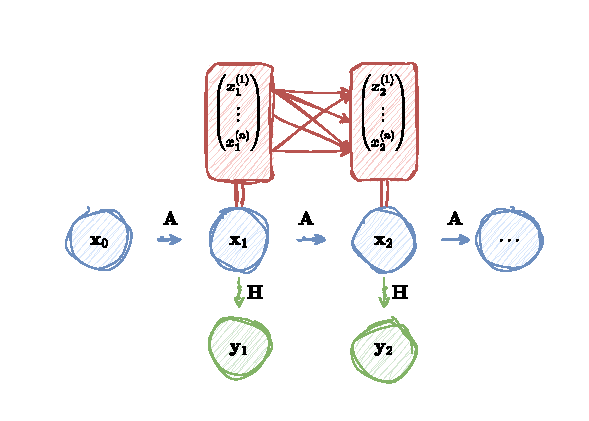
\includegraphics[width=0.75\linewidth]{fig/Markov Chian.pdf}
\caption{\textit{线性高斯状态空间模型}的流程。\textcolor{blue}{蓝色块}表示\textit{转换过程},\textcolor{red}{红色块}说明\textit{马尔可夫链属性}的细节,\textcolor{green}{绿色块}表示\textit{观察过程}。}
\label{fig: LGSSM 流程图}
\end{figure}

图~\ref{fig: LGSSM 流程图} 展示了线性高斯状态空间模型 (LGSSM) 的流程。蓝色块表示状态转换过程,描述系统随时间的变化。红色块突出了模型的马尔可夫属性,强调当前状态仅依赖于先前状态。绿色块表示观察过程,将状态映射到观察到的测量值。

\subsection{卡尔曼滤波器}
卡尔曼滤波器为线性高斯状态空间模型 (LGSSM) 中的状态估计问题提供了递归解决方案。卡尔曼滤波器涉及的关键分布是:
\begin{align}
 p(\mathbf{x}_k \mid \mathbf{y}_{1:k-1}) &\sim \mathcal{N}(\mathbf{x}_k \mid \mathbf{m}_k^-, \mathbf{P}_k^-), \\
 p(\mathbf{x}_k \mid \mathbf{y}_{1:k}) &\sim \mathcal{N}(\mathbf{x}_k \mid \mathbf{m}_k, \mathbf{P}_k), \\
 p(\mathbf{y}_k \mid \mathbf{y}_{1:k-1}) &\sim \mathcal{N}(\mathbf{y}_k \mid \mathbf{H}_k \mathbf{m}_k^-, \mathbf{S}_k)。\label{eq: single likelihood}
\end{align}

\subsubsection*{预测步骤}
预测步骤使用动态模型将状态估计及其不确定性从上一个时间步传播到当前时间步。预测步骤的公式如下:
\begin{align*}
\mathbf{m}_k^- &= \mathbf{A}_{k-1} \mathbf{m}_{k-1}, \\
\mathbf{P}_k^- &= \mathbf{A}_{k-1} \mathbf{P}_{k-1} \mathbf{A}_{k-1}^\mathsf{T} + \mathbf{Q}_{k-1}.
\end{align*}
其中,\(\mathbf{m}_k^-\) 和 \(\mathbf{P}_k^-\) 分别表示预测状态均值和协方差。

\subsubsection*{更新步骤}
更新步骤结合新的观测值 \(\mathbf{y}_k\) 来优化预测状态估计。更新步骤的方程为:
\begin{align}
 \mathbf{v}_k &= \mathbf{y}_k - \mathbf{H}_k \mathbf{m}_k^-, \label{eq: kalman filter vk} \\
 \mathbf{S}_k &= \mathbf{H}_k \mathbf{P}_k^- \mathbf{H}_k^\mathsf{T} + \mathbf{R}_k, \label{eq: kalman filter Sk} \\
 \mathbf{K}_k &= \mathbf{P}_k^- \mathbf{H}_k^\mathsf{T} \mathbf{S}_k^{-1}, \\
\mathbf{m}_k &= \mathbf{m}_k^- + \mathbf{K}_k \mathbf{v}_k, \\
\mathbf{P}_k &= \mathbf{P}_k^- - \mathbf{K}_k \mathbf{S}_k \mathbf{K}_k^\mathsf{T}.
\end{align}
其中,\(\mathbf{v}_k\) 为残差,\(\mathbf{S}_k\) 为残差协方差,\(\mathbf{K}_k\) 为卡尔曼增益,\(\mathbf{m}_k\) 和 \(\mathbf{P}_k\) 分别为更新后的状态均值和协方差。

\subsection{卡尔曼平滑器}
卡尔曼平滑器扩展了卡尔曼滤波器,它使用所有可用的观测值 \(\mathbf{y}_{1:T}\) 来估计每个时间步 \(k\) 的状态。具体来说,它计算平滑分布:
\begin{align*}
p(\mathbf{x}_k \mid \mathbf{y}_{1:T}) \sim \mathcal{N}(\mathbf{x}_k \mid \mathbf{m}_k^s, \mathbf{P}_k^s),
\end{align*}
其中 \(\mathbf{m}_k^s\) 和 \(\mathbf{P}_k^s\) 分别是平滑后的状态均值和协方差。

\subsubsection*{向后递归方程}
卡尔曼平滑器通过向后递归进行运算,从最终时间步长 \(T\) 开始,向后递归到初始时间步长 \(0\)。

\section{状态空间模型中的参数估计}
在贝叶斯框架中,缺失参数 \(\boldsymbol{\theta} \in \R^d\) 被视为具有先验分布 \(p(\boldsymbol{\theta})\) 的随机变量。包含这些缺失参数的状态空间模型 (SSM) 定义为:
\begin{align*}
\boldsymbol{\theta} &\sim p(\boldsymbol{\theta}), \\
\mathbf{x}_0 &\sim p(\mathbf{x}_0 \mid \boldsymbol{\theta}), \\
\mathbf{x}_k &\sim p(\mathbf{x}_k \mid \mathbf{x}_{k-1}, \boldsymbol{\theta}), \\
\mathbf{y}_k &\sim p(\mathbf{y}_k \mid \mathbf{x}_k, \boldsymbol{\theta})。
\end{align*}

参数估计的基本方法基于贝叶斯规则,该规则将给定观测值的状态和参数的联合后验分布表示为:
\begin{align*}
p(\mathbf{x}_{0:T}, \boldsymbol{\theta} \mid \mathbf{y}_{1:T}) = \frac{p(\mathbf{y}_{1:T} \mid \mathbf{x}_{0:T}, \boldsymbol{\theta}) \, p(\mathbf{x}_{0:T} \mid \boldsymbol{\theta}) \, p(\boldsymbol{\theta})}{p(\mathbf{y}_{1:T})},
\end{align*}
其中:
\begin{itemize}
\item \(p(\mathbf{x}_{0:T} \mid \boldsymbol{\theta}) = p(\mathbf{x}_0 \mid \boldsymbol{\theta}) \prod_{k=1}^{T} p(\mathbf{x}_k \mid \mathbf{x}_{k-1}, \boldsymbol{\theta})\) 是状态的先验分布,
\item \(p(\mathbf{y}_{1:T} \mid \mathbf{x}_{0:T}, \boldsymbol{\theta}) = \prod_{k=1}^{T} p(\mathbf{y}_k \mid \mathbf{x}_k, \boldsymbol{\theta})\) 是观测值。
\end{itemize}

参数估计的核心目标是找到最大化边缘后验分布的后验模态 \(\boldsymbol{\theta}\):
\begin{align*}
\boldsymbol{\theta} = \arg \max_{\boldsymbol{\theta}} p(\boldsymbol{\theta} \mid \mathbf{y}_{1:T})。
\end{align*}
这本质上是一个优化问题。然而,在解决这个问题之前,我们必须先解决计算 \(p(\boldsymbol{\theta} \mid \mathbf{y}_{1:T})\) 的难题。

为了集中计算 \(p(\boldsymbol{\theta} \mid \mathbf{y}_{1:T})\),即 \(\boldsymbol{\theta}\) 的边缘后验分布,直接求解方法涉及对状态进行边缘化:
\begin{align*}
p(\boldsymbol{\theta} \mid \mathbf{y}_{1:T}) = \int p(\mathbf{x}_{0:T}, \boldsymbol{\theta} \mid \mathbf{y}_{1:T}) \, \mathrm{d} \mathbf{x}_{0:T}.
\end{align*}

遗憾的是,计算这个高维积分极具挑战性,而且随着测量值的增多,计算难度也会越来越大。为了解决这个问题,我们提出了一些参数估计方法,该方法可以近似边缘后验分布 \(p(\boldsymbol{\theta} \mid \mathbf{y}_{1:T})\),而无需明确构建联合后验分布 \(p(\mathbf{x}_{0:T}, \boldsymbol{\theta} \mid \mathbf{y}_{1:T})\)。具体来说,我们关注:
\begin{align*}
p(\boldsymbol{\theta} \mid \mathbf{y}_{1:T}) \propto p(\mathbf{y}_{1:T} \mid \boldsymbol{\theta}) p(\boldsymbol{\theta})。
\end{align*}

因此,问题简化为计算 \textit{似然值} \(p(\mathbf{y}_{1:T} \mid \boldsymbol{\theta})\)。 (先验项 \(p(\boldsymbol{\theta})\) 是根据先验知识选择的,而归一化常数 \(p(\mathbf{y}_{1:T})\) 则被贝叶斯理论所避免。)

估计这种似然值的关键在于状态空间模型中的递归计算,也称为因式分解或预测误差分解:
\begin{align*}
p(\mathbf{y}_{1:T} \mid \boldsymbol{\theta}) = \prod^T_{k=1} p(\mathbf{y}_k \mid \mathbf{y}_{1:k-1}, \boldsymbol{\theta}),
\end{align*}
其中:
\begin{itemize}
\item \(p(\mathbf{y}_1 \mid \mathbf{y}_{1:0}, \boldsymbol{\theta}) \triangleq p(\mathbf{y}_1 \mid \boldsymbol{\theta})\)。
\end{itemize}

处理 \(p(\mathbf{y}_k \mid \mathbf{y}_{1:k-1}, \boldsymbol{\theta})\) 的核心思想是:
\begin{align*}
 p(\mathbf{y}_k \mid \mathbf{y}_{1:k-1}, \boldsymbol{\theta}) &= \int p(\mathbf{y}_k \mid \mathbf{x}_k, \boldsymbol{\theta}) \, p(\mathbf{x}_k \mid \mathbf{y}_{1:k-1}, \boldsymbol{\theta}) \, \mathrm{d} \mathbf{x}_k, \\
 p(\mathbf{x}_k \mid \mathbf{y}_{1:k}, \boldsymbol{\theta}) &= \frac{p(\mathbf{y}_k \mid \mathbf{x}_k, \boldsymbol{\theta}) \, p(\mathbf{x}_k \mid \mathbf{y}_{1:k-1}, \boldsymbol{\theta})}{p(\mathbf{y}_k \mid \mathbf{y}_{1:k-1}, \boldsymbol{\theta})},
\end{align*}
其中:
\begin{itemize}
 \item \(p(\mathbf{y}_k \mid \mathbf{x}_k, \boldsymbol{\theta})\) 是 \textit{测量模型},
 \item \(p(\mathbf{x}_k \mid \mathbf{y}_{1:k-1}, \boldsymbol{\theta})\) 是状态 \(\mathbf{x}_k\) 的 \textit{预测分布},由以下公式给出:
\begin{align*}
p(\mathbf{x}_k \mid \mathbf{y}_{1:k-1}, \boldsymbol{\theta}) = \int p(\mathbf{x}_k \mid \mathbf{x}_{k-1}, \boldsymbol{\theta}) p(\mathbf{x}_{k-1} \mid \mathbf{y}_{1:k-1}, \boldsymbol{\theta}) \, \mathrm{d} \mathbf{x}_{k-1}。
\end{align*}
\item \(p(\mathbf{x}_k \mid \mathbf{y}_{1:k}, \boldsymbol{\theta})\) 是 \textit{贝叶斯滤波器}。
\end{itemize}

注意,上述方程求解了状态空间模型中的似然函数。对于线性高斯状态空间模型的特殊情况,通过利用卡尔曼滤波器的结果,似然的计算得到了显著的简化。

\subsection{具有缺失参数的线性高斯状态空间模型}

具有缺失参数 \(\boldsymbol{\theta}\) 的线性高斯状态空间模型(LGSSM)定义为:
\begin{align*}
    \mathbf{x}_k &= \mathbf{A}(\boldsymbol{\theta}) \, \mathbf{x}_{k-1} + \mathbf{q}_{k-1}, \\
    \mathbf{y}_k &= \mathbf{H}(\boldsymbol{\theta}) \, \mathbf{x}_k + \mathbf{r}_k,
\end{align*}
其中:
\begin{itemize}
    \item \(\mathbf{q}_{k-1} \sim \mathcal{N}(\mathbf{0}, \mathbf{Q}(\boldsymbol{\theta}))\) 和 \(\mathbf{r}_{k} \sim \mathcal{N}(\mathbf{0}, \mathbf{R}(\boldsymbol{\theta}))\) 分别是过程噪声和测量噪声,
    \item \(\mathbf{x}_0 \sim \mathcal{N}(\mathbf{m}_0(\boldsymbol{\theta}), \mathbf{P}_0(\boldsymbol{\theta}))\) 是初始状态分布,
    \item 假设模型参数 \(\boldsymbol{\theta}\) 是时间不变的。
\end{itemize}

在接下来的章节中,我们将介绍应对 LGSSM 中计算和优化挑战的实用方法,具体包括梯度下降算法和期望最大化(EM)算法。

\subsection{梯度下降算法}

我们从方程~\eqref{eq: single likelihood} 中知道,\(p(\mathbf{y}_k \mid \mathbf{y}_{1:k-1}, \boldsymbol{\theta})\) 的分布是高斯分布:
\[
p(\mathbf{y}_k \mid \mathbf{y}_{1:k-1}, \boldsymbol{\theta}) \sim \mathcal{N}(\mathbf{H}_k(\boldsymbol{\theta}) \, \mathbf{m}_k^-(\boldsymbol{\theta}), \mathbf{S}_k(\boldsymbol{\theta})).
\]
因此,对数似然 \(\log p(\mathbf{y}_{1:T} \mid \boldsymbol{\theta})\) 可以表示为从正态分布推导出的递归求和项:
\begin{align*}
    \log p(\mathbf{y}_{1:T} \mid \boldsymbol{\theta}) = \sum^T_{k=1} \left( \frac{1}{2} \log | 2 \pi \, \mathbf{S}_k(\boldsymbol{\theta}) | + \frac{1}{2} \mathbf{v}_k^{\mathsf{T}}(\boldsymbol{\theta}) \, \mathbf{S}_k^{-1}(\boldsymbol{\theta}) \, \mathbf{v}_k (\boldsymbol{\theta}) \right),
\end{align*}
其中:
\begin{itemize}
    \item \(\mathbf{v}_k (\boldsymbol{\theta})\) 和 \(\mathbf{S}_k(\boldsymbol{\theta})\) 分别是残差值和残差协方差,定义见卡尔曼滤波器中的方程~\eqref{eq: kalman filter vk} 和方程~\eqref{eq: kalman filter Sk},
    \item \(m\) 是观测空间的维度,满足 \(\mathbf{y} \in \R^m\)。
\end{itemize}

令 \(\ell(\boldsymbol{\theta}) \triangleq \log p(\mathbf{y}_{1:T} \mid \boldsymbol{\theta})\)。为了最大化对数似然,我们使用梯度下降算法,该算法通过以下方式迭代更新参数估计 \(\boldsymbol{\theta}\):
\begin{align*}
    \boldsymbol{\theta}^{(i+1)} = \boldsymbol{\theta}^{(i)} - \eta \, \nabla_{\boldsymbol{\theta}} \ell(\boldsymbol{\theta}^{(i)}),
\end{align*}
其中:
\begin{itemize}
    \item \(\eta > 0\) 是学习率,控制更新的步长,
    \item \(\nabla_{\boldsymbol{\theta}} \ell(\boldsymbol{\theta})\) 是对数似然关于 \(\boldsymbol{\theta}\) 的梯度,
    \item \(\boldsymbol{\theta}^{(i)}\) 是第 \(i\) 次迭代中的参数估计。
\end{itemize}

梯度 \(\nabla_{\boldsymbol{\theta}} \ell(\boldsymbol{\theta})\) 可以使用链式法则计算,利用卡尔曼滤波器的递归性质。具体而言,\(\mathbf{v}_k(\boldsymbol{\theta})\) 和 \(\mathbf{S}_k(\boldsymbol{\theta})\) 的梯度项由卡尔曼滤波器方程推导得到,整体梯度通过求和所有时间步 \(k = 1, \dots, T\) 的贡献得到。

\subsection{EM 算法}
\paragraph*{状态空间模型的 EM 算法}
令 \(q(\mathbf{x}_{0:T})\) 为状态 \(\mathbf{x}_{0:T}\) 上的任意概率密度函数。对于对数似然 \(\log p(\mathbf{y}_{1:T} \mid \boldsymbol{\theta})\),总是存在一个下界,如下所示:
\begin{align}
    \log p(\mathbf{y}_{1:T} \mid \boldsymbol{\theta}) \ge F(q(\mathbf{x}_{0:T}), \boldsymbol{\theta}), \label{eq: ineq for EM}
\end{align}
其中二元函数 \(F(\cdot)\) 定义为:
\begin{align*}
    F(q(\mathbf{x}_{0:T}), \boldsymbol{\theta}) = \int q(\mathbf{x}_{0:T}, \boldsymbol{\theta}) \, \log \frac{p(\mathbf{x}_{0:T}, \mathbf{y}_{1:T} \mid \boldsymbol{\theta})}{q(\mathbf{x}_{0:T}, \boldsymbol{\theta})} \, \mathrm{d} \mathbf{x}_{0:T}.
\end{align*}

这自然引出了算法~\ref{alg: abstract EM},用于求解这个优化问题。

\begin{algorithm}[tb]
    \caption{简略 EM 算法}
    \label{alg: abstract EM}
    \begin{algorithmic}[1]
        \ENSURE{\(\boldsymbol{\theta}^{(N)}\)}
        \STATE \(\boldsymbol{\theta}^{(0)} \gets \text{随机值}\)
        \FOR{\(n = 0, 1, \dots, N-1\)}
            \STATE E 步骤:\(q^{(n+1)}(\cdot) \gets \arg \max_{q(\cdot)} F(q(\cdot), \boldsymbol{\theta}^{(n)})\)。
            \STATE M 步骤:\(\boldsymbol{\theta}^{(n+1)} \gets \arg \max_{\boldsymbol{\theta}} F(q^{(n+1)}(\cdot), \boldsymbol{\theta})\)。
        \ENDFOR
    \end{algorithmic}
\end{algorithm}

为了求解算法~\ref{alg: abstract EM} 中的 E 步骤,我们直接给出最优解:
\begin{align}
    q^{(n+1)}(\mathbf{x}_{0:T}) &= p(\mathbf{x}_{0:T} \mid \mathbf{y}_{1:T}, \boldsymbol{\theta}^{(n)}), \\
    F[q^{(n+1)}(\mathbf{x}_{0:T}), \boldsymbol{\theta}] &= \int p(\mathbf{x}_{0:T} \mid \mathbf{y}_{1:T}, \boldsymbol{\theta}^{(n)}) \log p(\mathbf{x}_{0:T}, \mathbf{y}_{1:T} \mid \boldsymbol{\theta}) \, \mathrm{d} \mathbf{x}_{0:T} \label{eq: full lower bound} \\
    &\quad - \int p(\mathbf{x}_{0:T} \mid \mathbf{y}_{1:T}, \boldsymbol{\theta}^{(n)}) \log p(\mathbf{x}_{0:T} \mid \mathbf{y}_{1:T}, \boldsymbol{\theta}^{(n)}) \, \mathrm{d} \mathbf{x}_{0{T}}. \nonumber
\end{align}

注意,方程~\eqref{eq: full lower bound} 中的第二项不依赖于 \(\boldsymbol{\theta}\)。因此,算法~\ref{alg: abstract EM} 中的 M 步骤优化可以简化,只考虑方程~\eqref{eq: full lower bound} 中的第一项作为对数似然的新下界,记作 \(\mathcal{Q}(\boldsymbol{\theta}, \boldsymbol{\theta}^{(n)})\):
\begin{align*}
    \mathcal{Q}(\boldsymbol{\theta}, \boldsymbol{\theta}^{(n)}) = \int p(\mathbf{x}_{0:T} \mid \mathbf{y}_{1:T}, \boldsymbol{\theta}^{(n)}) \log p(\mathbf{x}_{0:T}, \mathbf{y}_{1:T} \mid \boldsymbol{\theta}) \, \mathrm{d} \mathbf{x}_{0:T}.
\end{align*}

因此,我们得到了最终的迭代不等式,改编自方程~\eqref{eq: ineq for EM}:
\begin{align}
    \log p(\mathbf{y}_{1:T} \mid \boldsymbol{\theta}) \ge \mathcal{Q}(\boldsymbol{\theta}, \boldsymbol{\theta}^{(n)}). \label{eq: ineq for EM final}
\end{align}

这引出了简化版本的 EM 算法,用于估计状态空间模型的参数,如算法~\ref{alg: EM algorithm} 所示。

\begin{algorithm}[tb]
    \caption{状态空间模型的 EM 算法}
    \label{alg: EM algorithm}
    \begin{algorithmic}[1]
        \ENSURE{\(\boldsymbol{\theta}^{(N)}\)}
        \STATE \(\boldsymbol{\theta}^{(0)} \gets \text{随机值}\)
        \FOR{\(n = 0, 1, \dots, N-1\)}
            \STATE E 步骤:计算 \(\mathcal{Q}(\boldsymbol{\theta}, \boldsymbol{\theta}^{(n)})\)。
            \STATE M 步骤:\(\boldsymbol{\theta}^{(n+1)} \gets \arg \max_{\boldsymbol{\theta}} \mathcal{Q}(\boldsymbol{\theta}, \boldsymbol{\theta}^{(n)})\)。
        \ENDFOR
    \end{algorithmic}
\end{algorithm}

\paragraph*{线性高斯状态空间模型的 EM 算法}
在线性高斯状态空间模型(LGSSM)的假设下,\(\mathcal{Q}(\boldsymbol{\theta}, \boldsymbol{\theta}^{(n)})\) 的表达式为:
\begin{align}
    \mathcal{Q}(\boldsymbol{\theta}, \boldsymbol{\theta}^{(n)}) &= -\frac{1}{2} \log |2\pi \mathbf{P}_0(\boldsymbol{\theta})| - \frac{T}{2} \log |2\pi \mathbf{Q}(\boldsymbol{\theta})| - \frac{T}{2} \log |2\pi \mathbf{R}(\boldsymbol{\theta})| \nonumber \\
    &\quad - \frac{1}{2} \mathrm{tr} \left\{ \mathbf{P}_0^{-1}(\boldsymbol{\theta}) \left[ \mathbf{P}_0^s + (\mathbf{m}_0^s - \mathbf{m}_0(\boldsymbol{\theta}))(\mathbf{m}_0^s - \mathbf{m}_0(\boldsymbol{\theta}))^\mathsf{T} \right] \right\} \nonumber \\
    &\quad - \frac{T}{2} \mathrm{tr} \left\{ \mathbf{Q}^{-1}(\boldsymbol{\theta}) \left[ \boldsymbol{\Sigma} - \mathbf{C} \mathbf{A}^\mathsf{T}(\boldsymbol{\theta}) - \mathbf{A}(\boldsymbol{\theta}) \mathbf{C}^\mathsf{T} + \mathbf{A}(\boldsymbol{\theta}) \boldsymbol{\Phi} \mathbf{A}^\mathsf{T}(\boldsymbol{\theta}) \right] \right\} \nonumber \\
    &\quad - \frac{T}{2} \mathrm{tr} \left\{ \mathbf{R}^{-1}(\boldsymbol{\theta}) \left[ \mathbf{D} - \mathbf{B} \mathbf{H}^\mathsf{T}(\boldsymbol{\theta}) - \mathbf{H}(\boldsymbol{\theta}) \mathbf{B}^\mathsf{T} + \mathbf{H}(\boldsymbol{\theta}) \boldsymbol{\Sigma} \mathbf{H}^\mathsf{T}(\boldsymbol{\theta}) \right] \right\}, \label{eq: Q for LGSSM}
\end{align}
其中,中间量 \(\boldsymbol{\Sigma}, \boldsymbol{\Phi}, \mathbf{B}, \mathbf{C}, \mathbf{D}\) 计算为:
\begin{align}
    \boldsymbol{\Sigma} &= \frac{1}{T} \sum_{k=1}^{T} \mathbf{P}_k^s + \mathbf{m}_k^s [\mathbf{m}_k^s]^\mathsf{T}, \label{eq: middle Sigma} \\
    \boldsymbol{\Phi} &= \frac{1}{T} \sum_{k=1}^{T} \mathbf{P}_{k-1}^s + \mathbf{m}_{k-1}^s [\mathbf{m}_{k-1}^s]^\mathsf{T}, \label{eq: middle Phi} \\
    \mathbf{B} &= \frac{1}{T} \sum_{k=1}^{T} \mathbf{y}_k [\mathbf{m}_k^s]^\mathsf{T}, \label{eq: middle B} \\
    \mathbf{C} &= \frac{1}{T} \sum_{k=1}^{T} \mathbf{P}_k^s \mathbf{G}_{k-1}^\mathsf{T} + \mathbf{m}_k^s [\mathbf{m}_{k-1}^s]^\mathsf{T}, \label{eq: middle C} \\
    \mathbf{D} &= \frac{1}{T} \sum_{k=1}^{T} \mathbf{y}_k \mathbf{y}_k^\mathsf{T}, \label{eq: middle D}
\end{align}
这些量是由\textit{卡尔曼滤波器}和\textit{卡尔曼平滑器}的结果推导而来。

通过将梯度 \(\frac{\partial \mathcal{Q} (\boldsymbol{\theta}, \boldsymbol{\theta}^{(n)})}{\partial \boldsymbol{\theta}}\) 设置为零,我们得到以下闭式更新公式来更新参数:
\begin{align}
    \mathbf{m}_0^* &= \mathbf{m}_0^s, \label{eq: EM-M m0} \\
    \mathbf{P}_0^* &= \mathbf{P}_0^s + (\mathbf{m}_0^s - \mathbf{m}_0)(\mathbf{m}_0^s - \mathbf{m}_0)^{\mathsf{T}}, \label{eq: EM-M P0} \\
    \mathbf{A}^* &= \mathbf{C} \boldsymbol{\Phi}^{-1}, \label{eq: EM-M A} \\
    \mathbf{Q}^* &= \boldsymbol{\Sigma} - \mathbf{C} \mathbf{A}^{\mathsf{T}} - \mathbf{A} \mathbf{C}^{\mathsf{T}} + \mathbf{A} \boldsymbol{\Phi} \mathbf{A}^{\mathsf{T}}, \label{eq: EM-M Q} \\
    \mathbf{H}^* &= \mathbf{B} \boldsymbol{\Sigma}^{-1}, \label{eq: EM-M H} \\
    \mathbf{R}^* &= \mathbf{D} - \mathbf{H} \mathbf{B}^{\mathsf{T}} - \mathbf{B} \mathbf{H}^{\mathsf{T}} + \mathbf{H} \boldsymbol{\Sigma} \mathbf{H}^{\mathsf{T}}, \label{eq: EM-M R}
\end{align}
其中:
\begin{itemize}
    \item \(\boldsymbol{\theta}^*\) 表示 \(\arg \max_{\boldsymbol{\theta}} \mathcal{Q}(\boldsymbol{\theta}, \boldsymbol{\theta}^{(n)})\),对应算法~\ref{alg: EM algorithm} 中的 M 步骤。参数 \(\boldsymbol{\theta}\) 可以是 \(\{ \mathbf{A}, \mathbf{H}, \mathbf{Q}, \mathbf{R}, \mathbf{m}_0, \mathbf{P}_0 \}\) 的任意子集。
\end{itemize}

这引出了线性高斯状态空间模型的 EM 算法的实际实现,如算法~\ref{alg: EM algorithm for LGSSM} 所示。

\begin{algorithm}[h]
    \caption{线性高斯状态空间模型的 EM 算法}
    \label{alg: EM algorithm for LGSSM}
    \begin{algorithmic}[1]
        \ENSURE{\(\boldsymbol{\theta}^{(N)}\)}
        \STATE \(\boldsymbol{\theta}^{(0)} \gets \text{随机值}\)
        \FOR{\(n = 0, 1, \dots, N-1\)}
            \STATE E 步骤:使用卡尔曼滤波器和卡尔曼平滑器的结果计算 \(\boldsymbol{\Sigma}, \boldsymbol{\Phi}, \mathbf{B}, \mathbf{C}, \mathbf{D}\),并使用 \(\boldsymbol{\theta}^{(n)}\)。
            \STATE M 步骤:使用方程~\eqref{eq: EM-M A}, \eqref{eq: EM-M H}, \eqref{eq: EM-M Q}, \eqref{eq: EM-M R}, \eqref{eq: EM-M m0}, 和 \eqref{eq: EM-M P0} 更新 \(\boldsymbol{\theta}^{(n+1)} \gets \arg \max_{\boldsymbol{\theta}} \mathcal{Q}(\boldsymbol{\theta}, \boldsymbol{\theta}^{(n)})\)。
        \ENDFOR
    \end{algorithmic}
\end{algorithm}

\newclearpage
% \chapter{基于卷积神经的手写数字及写字人识别算法设计}
% \section{输入输出层的设计}
% \section{隐藏层的设计}
% \section{本章小结}

\chapter{GraphEM 算法}

\section{引言}

本节中,我们提出了一个通用框架,用于在适当的先验假设下估计线性高斯状态空间模型(LGSSM)的转移矩阵 \(\mathbf{A}\)。我们的目标是寻找 \(\widehat{\mathbf{A}}\),使得:
\begin{align}
    \widehat{\mathbf{A}} = \arg \max_{\mathbf{A}} p(\mathbf{A} \mid \mathbf{y}_{1:T}), \label{eq: GraphEM argmax}
\end{align}
其中:
\begin{itemize}
    \item 由贝叶斯法则得:\(p(\mathbf{A} \mid \mathbf{y}_{1:T}) \propto p(\mathbf{y}_{1:T} \mid \mathbf{A}) p(\mathbf{A})\)。
\end{itemize}

回忆在未引入先验信息之前,对数似然函数的下界由式~\eqref{eq: ineq for EM final}给出:
\begin{align}
    \log p(\mathbf{y}_{1:T} \mid \mathbf{A}) \ge \mathcal{Q}(\mathbf{A}, \mathbf{A}^{(n)})。
\end{align}

为了引入先验信息,我们为 EM 框架导出一个新的下界:
\begin{align}
    \log p(\mathbf{y}_{1:T} \mid \mathbf{A}) + \log p(\mathbf{A}) \ge \mathcal{Q}(\mathbf{A}, \mathbf{A}^{(n)}) + \log p(\mathbf{A})。 \label{eq: ineq for GraphEM}
\end{align}

为适应最小化问题,我们引入新的记号。令损失函数为负对数似然:
\begin{align}
    \mathcal{L}_T(\mathbf{A}) \triangleq \mathcal{L}_0(\mathbf{A}) + \mathcal{L}_{1:T}(\mathbf{A}),
\end{align}
其中:
\begin{itemize}
    \item \(\mathcal{L}_0(\mathbf{A}) = -\log p(\mathbf{A})\) 是先验损失项,
    \item \(\mathcal{L}_{1:T}(\mathbf{A}) = -\log p(\mathbf{y}_{1:T} \mid \mathbf{A})\) 是似然损失项。
\end{itemize}

采用该记号,我们的优化目标可由式~\eqref{eq: GraphEM argmax}重写为:
\begin{align}
    \widehat{\mathbf{A}} = \arg \min_{\mathbf{A}} \mathcal{L}_T(\mathbf{A})。
\end{align}

我们引入一个新的上界作为 GraphEM 算法中的目标函数:
\begin{align}
    \mathfrak{Q}(\mathbf{A}, \mathbf{A}^{(n)}) \triangleq -\mathcal{Q}(\mathbf{A}, \mathbf{A}^{(n)}) + \lambda \, \mathcal{L}_0(\mathbf{A}), \label{eq: new upper bound for GraphEM}
\end{align}
其中 \(\lambda\) 用于控制先验损失项 \(\mathcal{L}_0(\mathbf{A})\) 的权重。

利用新记号重写式~\eqref{eq: ineq for GraphEM},并改变不等号方向,可得上界形式的 EM 结构:
\begin{align}
    \mathcal{L}_T(\mathbf{A}) \le \mathfrak{Q}(\mathbf{A}, \mathbf{A}^{(n)})。
\end{align}

采用目标函数 \(\mathfrak{Q}(\mathbf{A}, \mathbf{A}^{(n)})\),我们提出 GraphEM 算法,如算法~\ref{alg: abstract GraphEM algorithm} 所示。

\begin{algorithm}[tb]
    \caption{简略 GraphEM 算法}
    \label{alg: abstract GraphEM algorithm}
    \begin{algorithmic}[1]
        \ENSURE{\(\mathbf{A}^{(N)}\)}
        \STATE \(\mathbf{A}^{(0)} \gets \text{随机初始化}\)
        \FOR{\(n = 0, 1, \dots, N-1\)}
            \STATE E 步骤:计算 \(\mathfrak{Q}(\mathbf{A}, \mathbf{A}^{(n)})\)。
            \STATE M 步骤:\(\mathbf{A}^{(n+1)} \gets \arg \min_{\mathbf{A}} \mathfrak{Q}(\mathbf{A}, \mathbf{A}^{(n)})\)。
        \ENDFOR
    \end{algorithmic}
\end{algorithm}

\section{E 步骤中的计算}

本节中,我们专注于计算目标函数 \(\mathfrak{Q}(\mathbf{A}, \mathbf{A}^{(n)})\)。

回忆,对于线性高斯状态空间模型(LGSSM),下界 \(\mathcal{Q}(\mathbf{A}, \mathbf{A}^{(n)})\) 由式~\eqref{eq: Q for LGSSM}给出。由于我们只关心 \(\mathbf{A}\),该表达式可简化为:
\begin{align}
    \mathcal{Q}(\mathbf{A}, \mathbf{A}^{(n)}) = - \frac{T}{2} \tr \left\{ \mathbf{Q}^{-1} \left[ \boldsymbol{\Sigma} - \mathbf{C} \mathbf{A}^{\mathsf{T}} - \mathbf{A} \mathbf{C}^{\mathsf{T}} + \mathbf{A} \boldsymbol{\Phi} \mathbf{A}^{\mathsf{T}} \right] \right\} + \constA,
\end{align}
其中:
\begin{itemize}
    \item \(\boldsymbol{\Sigma} = \boldsymbol{\Sigma}(\mathbf{A}^{(n)})\),由式~\eqref{eq: middle Sigma} 计算,
    \item \(\boldsymbol{\Phi} = \boldsymbol{\Phi}(\mathbf{A}^{(n)})\),由式~\eqref{eq: middle Phi} 计算,
    \item \(\mathbf{C} = \mathbf{C}(\mathbf{A}^{(n)})\),由式~\eqref{eq: middle C} 计算,
    \item \(\constA\) 表示与 \(\mathbf{A}\) 无关的常数项。
\end{itemize}

利用式~\eqref{eq: new upper bound for GraphEM},一旦评估出 \(\mathcal{L}_0(\mathbf{A})\),我们便可以计算 \(\mathfrak{Q}(\mathbf{A}, \mathbf{A}^{(n)})\)。这完成了 E 步骤中目标函数的计算。

\section{M 步骤中的优化}

本节的目标是找到使目标函数 \(\mathfrak{Q}(\mathbf{A}, \mathbf{A}^{(n)})\) 最小化的矩阵 \(\mathbf{A}\)。

在标准的 EM 算法中,该优化问题通常具有闭式解。然而,在我们的目标函数中引入了先验项,使问题变得更加复杂,因此需要采用专门的优化方法。这里,我们提出一种适用于该修正 EM 结构的求解方法。

\subsection{近端算子}

设 \( f: \mathbb{R}^{n \times n} \to \mathbb{R} \) 是一个适当的、凸的、下半连续的函数。函数 \( f \) 在点 \(\tilde{\mathbf{A}} \in \mathbb{R}^{n \times n}\) 的\textit{近端算子}定义为:
\begin{align}
    \text{prox}_{f}(\tilde{\mathbf{A}}) = \arg\min_{\mathbf{A}} \left( f(\mathbf{A}) + \frac{1}{2} \| \mathbf{A} - \tilde{\mathbf{A}} \|^2_F \right)。
\end{align}

我们的目标函数由两项组成。首先,我们推导第一项 \(-\mathcal{Q}(\mathbf{A}, \mathbf{A}^{(n)})\) 的近端算子,其形式如下:
\begin{align}
    \mathrm{prox}_{-\vartheta\mathcal{Q}(\tilde{\mathbf{A}}, \mathbf{A}^{(n)})} (\tilde{\mathbf{A}}) = \mathrm{lyapuov} \left( \vartheta \mathbf{Q}^{-1}, \boldsymbol{\Phi}^{-1}, \tilde{\mathbf{A}} \boldsymbol{\Phi}^{-1} + \vartheta \mathbf{Q}^{-1} \mathbf{C} \boldsymbol{\Phi}^{-1} \right),
\end{align}
其中:
\begin{itemize}
    \item \(\vartheta > 0\) 是缩放参数,
    \item \(\mathrm{lyapuov}(X, Y, Z)\) 表示 Lyapunov 方程 \(XW + WY = Z\) 的解。
\end{itemize}

进一步地,若 \(\mathbf{Q} = \mathbf{I}_{n} \sigma^2_{\mathbf{Q}}\),则近端算子可简化为:
\begin{align}
    \mathrm{prox}_{-\vartheta\mathcal{Q}(\tilde{\mathbf{A}}, \mathbf{A}^{(n)})} (\tilde{\mathbf{A}}) = \left( \frac{\vartheta\, T}{\sigma^2_{\mathbf{Q}}} \mathbf{C} + \tilde{\mathbf{A}} \right) \left( \frac{\vartheta}{\sigma^2_{\mathbf{Q}}} \boldsymbol{\Phi} + \mathbf{I}_{n} \right)^{-1},
\end{align}
其中:
\begin{itemize}
    \item \(\sigma^2_{\mathbf{Q}} > 0\) 是过程噪声的方差,
    \item \(I_{n} \in \mathbb{R}^{n \times n}\) 是单位矩阵。
\end{itemize}

\subsection{Douglas-Rachford 迭代法}

我们考虑如下优化问题:
\begin{equation}
    \min_{\mathbf{A}} \mathfrak{Q}(\mathbf{A}, \mathbf{A}^{(n)}) \equiv \min_{\mathbf{A}} -\mathcal{Q}(\mathbf{A}, \mathbf{A}^{(n)}) + \mathcal{L}_0(\mathbf{A})。
\end{equation}

通过定义:
\begin{equation}
    f_1(\mathbf{A}) \triangleq -\mathcal{Q}(\mathbf{A}, \mathbf{A}^{(n)}), \quad f_2(\mathbf{A}) \triangleq \mathcal{L}_0(\mathbf{A}),
\end{equation}
该问题可以使用 Douglas-Rachford 迭代法求解,其形式如下:
\begin{equation}
    \mathbf{A}^{(i+1)} = \mathbf{A}^{(i)} + \alpha \left( \operatorname{prox}_{\vartheta f_1} \big(2 \operatorname{prox}_{\vartheta f_2}(\mathbf{A}^{(i)}) - \mathbf{A}^{(i)} \big) - \operatorname{prox}_{\vartheta f_2}(\mathbf{A}^{(i)}) \right),
\end{equation}
其中我们设置 \(\alpha = 1\)。

在我们的具体问题中,两个近端算子分别为:
\begin{align}
    \operatorname{prox}_{\vartheta f_1}(\mathbf{A}^{(i)}) &\triangleq \arg\min_{\mathbf{A}} \left( -\mathcal{Q}(\mathbf{A}, \mathbf{A}^{(n)}) + \frac{1}{2\vartheta} \| \mathbf{A} - \mathbf{A}^{(i)} \|^2 \right), \\
    \operatorname{prox}_{\vartheta f_2}(\mathbf{A}^{(i)}) &\triangleq \arg\min_{\mathbf{A}} \left( \mathcal{L}_0(\mathbf{A}) + \frac{1}{2\vartheta} \| \mathbf{A} - \mathbf{A}^{(i)} \|^2 \right),
\end{align}
其中 \(\operatorname{prox}_{\vartheta f_1}(\mathbf{A}^{(i)})\) 和 \(\operatorname{prox}_{\vartheta f_2}(\mathbf{A}^{(i)})\) 的计算方法可参考前一节以及表~\ref{tab: reg prox table}。

Douglas-Rachford 方法在解决结构化优化问题中表现出色,适用于凸和非凸场景。用于 M 步优化的显式迭代步骤列于算法~\ref{alg: Douglas-Rachford} 中。

\begin{algorithm}[tb]
    \caption{M 步中的 Douglas-Rachford 迭代法}
    \label{alg: Douglas-Rachford}
    \begin{algorithmic}[1]
        \ENSURE{\(\mathbf{A}^{(n+1)}\).}
        \STATE \(\mathbf{A}^{(0)} \gets \mathbf{A}^{(n)}\)。
        \FOR{\(i = 0, 1, 2, \dots\)}
            \STATE 计算 \(\mathbf{Y}^{(i)} = \operatorname{prox}_{\vartheta f_2}(\mathbf{A}^{(i)})\)。
            \STATE 计算 \(\mathbf{Z}^{(i)} = \operatorname{prox}_{\vartheta f_1}(2\mathbf{Y}^{(i)} - \mathbf{A}^{(i)})\)。
            \STATE 更新 \(\mathbf{A}^{(i+1)} \gets \mathbf{A}^{(i)} + \lambda (\mathbf{Z}^{(i)} - \mathbf{Y}^{(i)})\)。 
        \ENDFOR
        \STATE \(\mathbf{A}^{(n+1)} \gets \mathbf{A}^{(i)}\)。
    \end{algorithmic}
\end{algorithm}

\section{先验正则化}

在 GraphEM 算法中,先验正则化在优化过程中起着关键作用,有助于提升稳定性和性能。本节将介绍用于算法中的稳定性约束及多种可选的正则项。这些约束与正则项对于引导优化方向至关重要,能够确保转移矩阵 \(\mathbf{A}\) 满足期望的性质,如稀疏性、平滑性或结构限制等。

\subsection{稳定性约束}

为了确保算法的稳定性,我们对初始转移矩阵 \(\mathbf{A}\) 施加约束。具体而言,我们要求 \(\mathbf{A}\) 的谱范数被一个常数 \(\delta < 1\) 所约束。该约束确保系统动力学保持稳定,并使优化过程具有良好的收敛性。约束集合 \(\mathcal{S}\) 定义如下:
\begin{align}
    \mathcal{S} = \left\{ \mathbf{A} \in \mathbb{R}^{n \times n} \mid \| \mathbf{A} \|_2 \le \delta < 1 \right\},
\end{align}
其中 \(\delta \in (0, 1)\) 是用户设定的参数,用于控制系统的稳定性。

表~\ref{tab: convex constrain table} 给出了常见凸约束集合的示例及其对应的投影算子。这些约束对于在优化过程中保持转移矩阵 \(\mathbf{A}\) 位于可行区域内至关重要。

\begin{table}[tb]
    \centering
    \caption{常见凸约束集合及其投影算子示例。}
    \label{tab: convex constrain table}
    \begin{tabular}{lll}
        \toprule
        \textbf{约束类型} & \(\mathcal{S}\) & \(\mathrm{Proj}_\mathcal{S} (\mathbf{A})\) \\
        \midrule
        谱范数约束 & \(\| \mathbf{A} \|_2 \le \delta\) & \(\mathbf{U}^{\mathsf{T}} \mathrm{diag}\left( \left( \mathrm{sign}(s_i) \min(|s_i|, \delta) \right)_{i \le n} \right) \mathbf{V}\) \\
        \addlinespace
        元素范围约束 & \(\left( a_{ij} \in [a_{\min}, a_{\max} ] \right)_{i, j\le n}\) & \(\left( \min \left( \max \left( a_{ij}, a_{\min} \right) , a_{\max} \right) \right)_{i, j \le n}\) \\
        \addlinespace
        Frobenius 范数约束 & \(\| \mathbf{A} \|_F \le \delta\) & \(\left( a_{ij}(1 - \frac{\delta}{\max (\| \mathbf{A} \|_F, \delta)}) \right)_{i, j \le n}\) \\
        \bottomrule
    \end{tabular}
\end{table}

\subsection{正则项}

除了稳定性约束外,我们还引入惩罚项以对转移矩阵 \(\mathbf{A}\) 进行正则化。这些惩罚项来源于对 \(\mathbf{A}\) 结构的先验知识,并以 \(\mathcal{L}_0(\mathbf{A})\) 的形式融入目标函数中。不同的正则项鼓励 \(\mathbf{A}\) 具备不同的性质,例如稀疏性、块稀疏性或平滑性等。

表~\ref{tab: reg prox table} 列举了常用的先验类型、对应的正则项 \(\mathcal{L}_0(\mathbf{A})\) 及其相关的近端算子。这些正则项在引导优化过程中发挥着关键作用,确保所估计的转移矩阵 \(\mathbf{A}\) 与其潜在图结构保持一致。

\begin{table}[tb]
    \centering
    \caption{先验类型、正则项及其在尺度参数 \(\vartheta > 0\) 下的近端算子示例。}
    \label{tab: reg prox table}
    \begin{tabular}{@{}p{1.8cm}p{4.1cm}p{8cm}@{}}
        \toprule
        \textbf{先验类型} & \textbf{\(\mathcal{L}_0(\mathbf{A})\)} & \textbf{\(\text{prox}_{\vartheta \mathcal{L}_0}(\mathbf{A})\)} \\ 
        \midrule
        Laplace & \(\|\mathbf{A}\|_1\) & \(\left(\text{sign}(a_{ij}) \max(0, |a_{ij}| - \lambda\vartheta)\right)_{i, j \le n}\) \\ 
        \addlinespace
        Block-Laplace & \(\|\mathbf{A}\|_{2, 1} = \sum_{b=1}^B \|\mathbf{a}(b)\|_2\) & \(\left(\left(1 - \frac{\lambda\vartheta}{\max(\|\mathbf{a}(b)\|_2, \lambda\vartheta)}\right)\mathbf{a}(b)\right)_{b \le B}\) \\ 
        \addlinespace
        Gaussian & \(\frac{1}{2} \|\mathbf{A}\|_F^2\) & \(\left(\frac{a_{ij}}{1+\lambda\vartheta}\right)_{i, j \le n}\) \\ 
        \addlinespace
        Laplace + Gaussian & \(\|\mathbf{A}\|_1 + \frac{1}{2} \|\mathbf{A}\|_F^2\) & \(\left(\text{sign}\left(\frac{a_{ij}}{1+\lambda\vartheta}\right) \max\left(0, |\frac{a_{ij}}{1+\lambda\vartheta}| - \frac{\lambda\vartheta}{1+\lambda\vartheta}\right)\right)_{i, j \le n}\) \\ 
        \bottomrule
    \end{tabular}
\end{table}

稳定性约束与正则项对于确保 GraphEM 算法产生具有意义且可解释的结果至关重要。稳定性约束保证了系统动力学的稳定性,而正则项则融入了关于转移矩阵 \(\mathbf{A}\) 结构的先验知识。

这些先验在处理不同类型图结构时尤其有用,例如小世界网络、无标度网络或二部图等,有助于算法适应图结构的特定性质。这种适配性使得算法能够有效捕捉图中节点之间的复杂关系,从而提升推断的准确性。

通过结合稳定性约束与正则项,GraphEM 算法为估计转移矩阵提供了一个灵活的框架,可广泛应用于时间序列分析、网络推断等多个领域。正则项的选择依赖于具体问题和对转移矩阵性质的需求,从而使该算法能够高度适配不同应用场景,尤其是在面对具有不同连接模式和拓扑结构的图时,能够更精确地捕捉潜在的动态过程。


\newclearpage
% \chapter{第四章	手写数字及写字人识别实验过程及其结果}
% \section{手写数字识别实验}
% \subsection{样本简介}

% 本论文的手写数字识别实验当中所用的样本分为两类,一类是训练样本集,另一类是测试样本集。
% 实验当中的训练样本集采用的是手写数字MNIST数据库。这个数据库当中包含训练集样本60000个样例和测试集样本10000个样例。MNIST数据库当中的数字样本已经全部大小归一化灰度化并且集中到同一个固定大小的图像当中。该数据库包括MST的SD-1和SD-3数据库,当中包含一系列的二级制的手写数字图像。其中SD-1的收集者来源是某高中的在校学生,而SD-3是由人口调查局员工收集的。则我们的训练样本集也就是MNIST当中的训练样本集有30000个样本来自SD-3,而另外30000个样本来自SD-1。这60000个训练样本分别来自约250个采集者。
% \subsection{Writer Depend类数字识别实验}
% \subsubsection{ABCvsA数字识别实验}
% 实验内容:以A写字人、B写字人和C写字人,合计3000个数字0到9的数字图像数据为训练样本集。A写字人的1000个数字0到9的数字图像数据为测试样本集。学习率为1,单次训练样本数为10个,共训练40次。若识别所得数字与给定的标签匹配,则视为正确;不匹配则视为错误。
% \begin{table}[htbp]
%     \centering
%     \caption{ABCvsA数字识别实验结果}
%     \label{tab:1}
%     \begin{tabular}{@{}cccc@{}}
%         \toprule
%         训练样本 & ABC & 样本个数    & 3000    \\ \midrule
%         测试样本 & A   & 样本个数    & 1000    \\
%         训练次数 & —   & 单次训练样本数 & 10      \\
%         学习率  & 1   & 正确率     & 99.50\% \\ \bottomrule
%     \end{tabular}
% \end{table}

% \subsubsection{ABCvsABC数字识别实验}
% 实验内容:以A写字人、B写字人和C写字人,合计3000个数字0到9的数字图像数据为总样本集。在总样本集当中随机抽取2400个为训练样本集,余下的600个为测试样本集。学习率为1,单次训练样本数为10个,共训练40次。若识别所得数字与给定的标签匹配,则视为正确;不匹配则视为错误。
% \begin{table}[htbp]
%     \centering
%     \caption{ABCvsABC数字识别实验结果}
%     \label{tab:2}
%     \begin{tabular}{@{}cccc@{}}
%         \toprule
%         训练样本 & ABC & 样本个数    & 2400    \\ \midrule
%         测试样本 & ABC & 样本个数    & 600     \\
%         训练次数 & 40  & 单次训练样本数 & 10      \\
%         学习率  & 1   & 正确率     & 92.00\% \\ \bottomrule
%     \end{tabular}
% \end{table}
% \subsection{Writer Depend类数字识别实验结果分析}

% 下面我们选取Writer Depend类数字识别实验当中的两个典型的例子ABCvsA数字识别实验以及MNIST\&ABCvsA数字识别实验的结果做详细分析。我们从ABCvsA数字识别实验中的训练样本集和测试样本集的手写数字图像样本集当中分别随机抽取一幅图像\ref{fig:complex}所示。

% \begin{figure}[htbp] % image examples & compare
%     \begin{subfigure}{0.5\textwidth}
%         \centering
%         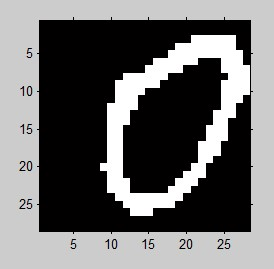
\includegraphics[height=6.54cm]{image/chap04/1.jpg}
%         \caption{实验训练集}
%         \label{fig:compare1}
%     \end{subfigure}
%     \begin{subfigure}{0.5\textwidth}
%         \centering
%         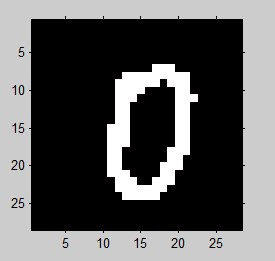
\includegraphics[height=6.54cm]{image/chap04/2.jpg}
%         \caption{实验测试集}
%         \label{fig:compare2}
%     \end{subfigure}
%     \caption{ABCvsA数字识别实验集}
%     \label{fig:complex}
% \end{figure}

% 下面我们对上述的训练集和测试集进行40次学习率为2,单次训练样本为10的迭代,得到错误率为0.50\%,而其中每次训练时的误差值组成的历史误差值画图分析如下:
% ……
% \subsection{Writer Independ类数字识别实验}
% 实验内容:以MNIST数据库为训练样本集,共计60000个训练样本。以A写字人合计1000个数字0到9的数字图像数据为测试样本集写字人识别实验
% ……
% \subsection{样本简介}
% ……
% \subsection{两位写字人识别实验}
% \subsubsection{单个数字的写字人识别实验}
% 实验内容:以A写字人,合计800个数字5的数字图像数据加上B写字人,合计800个数字5的数字图像数据,共计1600个样本为总样本集。随机选取其中的1200个样本为训练样本集,其余的400个样本为测试样本集。学习率为2,单次训练样本数为10个,共训练30次。若识别所得写字人与给定的标签匹配,则视为正确;不匹配则视为错误。
% \begin{table}[]
%     \centering
%     \caption{单个数字写字人识别实验结果}
%     \label{tab:3}
%     \begin{tabular}{@{}cccc@{}}
%         \toprule
%         训练样本 & A5\&B5 & 样本个数    & 1200    \\ \midrule
%         测试样本 & A5\&B5 & 样本个数    & 400     \\
%         训练次数 & 30     & 单次训练样本数 & 10      \\
%         学习率  & 2      & 正确率     & 99.75\% \\ \bottomrule
%     \end{tabular}
% \end{table}
% \subsubsection{单个数字的写字人识别实验结果分析}

% ……
% \section{本章小结}

% ……。

\chapter{数值实验}

\section{汽车的动态模型}

在本节中,我们通过一个真实场景示例展示卡尔曼滤波器的强大能力及其捕捉马尔可夫过程行为的效果。我们考虑一个汽车的动态模型,该模型在二维坐标系中模拟汽车的运动,并跟踪其位置与速度。转移矩阵 \(\mathbf{A}\) 定义如下:

\begin{align}
    \begin{pmatrix}
        x_k^{(1)} \\
        x_k^{(2)} \\
        x_k^{(3)} \\
        x_k^{(4)}
    \end{pmatrix} = \underbrace{
    \begin{pmatrix}
    1 & 0 & \Delta t & 0 \\
    0 & 1 & 0 & \Delta t \\
    0 & 0 & 1 & 0 \\
    0 & 0 & 0 & 1
    \end{pmatrix}}_{\mathbf{A}}
    \begin{pmatrix}
    x_{k-1}^{(1)} \\
    x_{k-1}^{(2)} \\
    x_{k-1}^{(3)} \\
    x_{k-1}^{(4)}
    \end{pmatrix}
    +
    \mathbf{q}_{k-1}, \label{eq: exp car A}
\end{align}

其中 \(\mathbf{q}_{k-1}\) 是一个离散时间高斯噪声过程,其均值为零,协方差矩阵 \(\mathbf{Q}\) 定义为:

\begin{align}
    \mathbf{Q} = 
    \begin{pmatrix}
    \frac{q_{1}^c \Delta t^3}{3} & 0 & \frac{q_{1}^c \Delta t^2}{2} & 0 \\
    0 & \frac{q_{2}^c \Delta t^3}{3} & 0 & \frac{q_{2}^c \Delta t^2}{2} \\
    \frac{q_{1}^c \Delta t^2}{2} & 0 & q_{1}^c \Delta t & 0 \\
    0 & \frac{q_{2}^c \Delta t^2}{2} & 0 & q_{2}^c \Delta t
    \end{pmatrix}.
\end{align}

该动态系统的线性高斯状态空间模型(LGSSM)完整形式为:

\begin{align}
    \mathbf{x}_k &= \mathbf{A}_{k-1} \mathbf{x}_{k-1} + \mathbf{q}_{k-1}, \\
    \mathbf{y}_k &= \mathbf{H}_k \mathbf{x}_{k} + \mathbf{r}_{k},
\end{align}

其中模型参数设置如下:
\begin{itemize}
    \item \(\mathbf{A}_{k-1}\) 按照式~\eqref{eq: exp car A} 定义,
    \item \(\mathbf{H}_k = \mathbf{I}_4\),
    \item \(\mathbf{r}_k \sim \mathcal{N}(\mathbf{0}, \sigma_\mathbf{r}^2 \mathbf{I}_4)\),其中 \(\sigma_\mathbf{r} = 0.1\),
    \item \(\mathbf{x}_0 \sim \mathcal{N}(\mathbf{m}_0, \mathbf{P}_0)\),其中 \(\mathbf{m}_0 = \mathbf{0}\),\(\mathbf{P}_0 = \sigma_\mathbf{P}^2 \mathbf{I}_4\),\(\sigma_\mathbf{P} = 0.1\)。
\end{itemize}

该模型表示的是匀速运动,其中状态向量的前两个分量对应位置,后两个分量对应速度。卡尔曼滤波器与平滑器为估计观测数据背后的潜在状态变量提供了闭式解法。

\begin{figure}
    \centering
    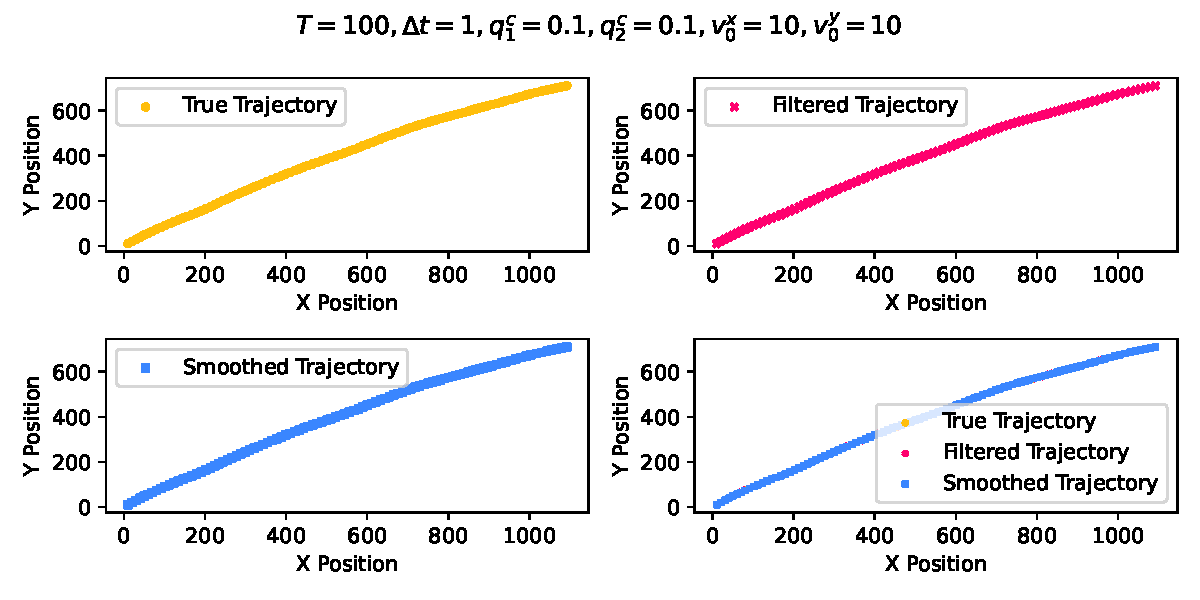
\includegraphics[width=0.95\linewidth]{fig/estimated_car_trajectory.pdf}
    \caption{观测轨迹与使用卡尔曼滤波器和平滑器估计得到的轨迹。}
    \label{fig: exp car trajectory}
\end{figure}

图~\ref{fig: exp car trajectory} 展示了实验结果,绘制了使用卡尔曼滤波器和平滑器所估计的轨迹。该图直观展示了这些方法在准确估计潜在状态变量方面的有效性。

我们还使用经典的期望最大化(EM)算法对该汽车模型的参数进行估计。EM 算法是状态空间模型中广泛应用的参数估计方法,我们将在该示例中评估其性能。

\begin{table}[tb]
\centering
\caption{汽车模型的 EM 算法结果。基线负对数似然为 \(\mathcal{L}_T({\boldsymbol{\theta}}) = -261.989\)。}
\label{tab: exp car EM results}
\begin{tabular}{lll}
\toprule
\textbf{待估参数} & \textbf{\(\mathcal{L}_T(\widehat{\boldsymbol{\theta}})\)} & \textbf{\(\| \widehat{\boldsymbol{\theta}} - \boldsymbol{\theta} \|_F\)} \\
\midrule
\(\mathbf{A}\) & -273.250 & 0.248 \\
\(\mathbf{Q}\) & -247.424 & 0.308 \\
\(\mathbf{H}\) & -169.839 & 0.642 \\
\bottomrule
\end{tabular}
\end{table}

表~\ref{tab: exp car EM results} 总结了使用 EM 算法对参数 \(\mathbf{A}\)、\(\mathbf{Q}\) 和 \(\mathbf{H}\) 的估计结果。表中列出了每个估计参数对应的负对数似然值 \(\mathcal{L}_T(\widehat{\boldsymbol{\theta}})\) 以及与真实参数之间的 Frobenius 范数 \(\| \widehat{\boldsymbol{\theta}} - \boldsymbol{\theta} \|_F\)。

\begin{figure}[tb]
    \centering
    \begin{subfigure}[b]{0.95\textwidth}
        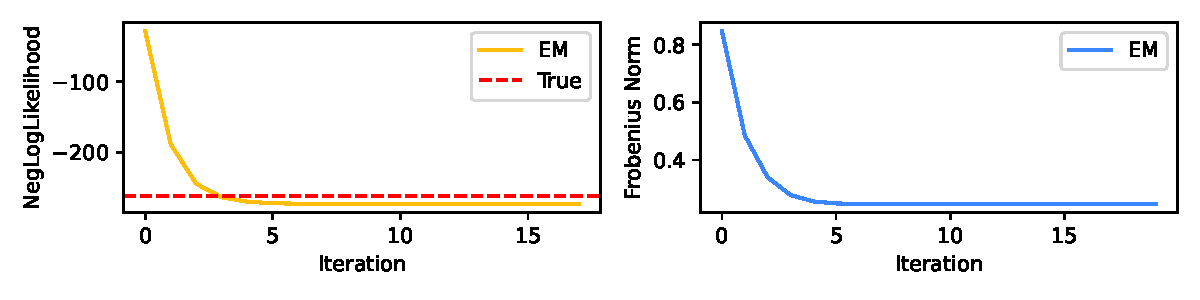
\includegraphics[width=\textwidth]{fig/A_neg_log_likelihood_fnorm.pdf}
        \caption{\(\mathbf{A}\) 的负对数似然与 Frobenius 范数变化。}
        \label{fig:subfig1}
    \end{subfigure}
    
    \begin{subfigure}[b]{0.95\textwidth}
        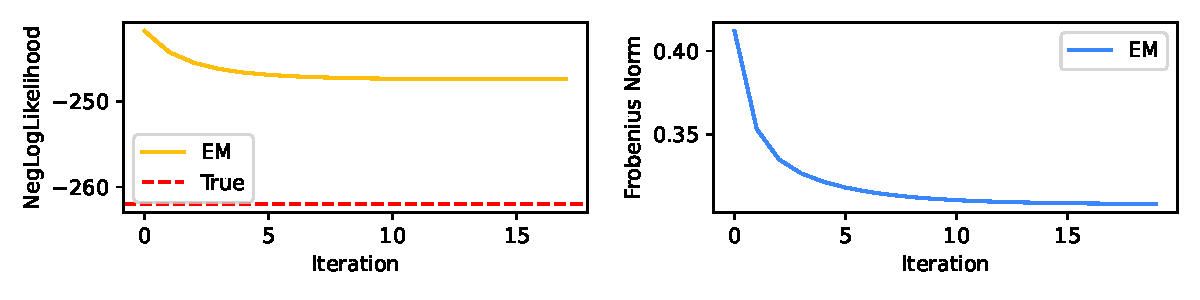
\includegraphics[width=\textwidth]{fig/Q_neg_log_likelihood_fnorm.pdf}
        \caption{\(\mathbf{Q}\) 的负对数似然与 Frobenius 范数变化。}
        \label{fig:subfig2}
    \end{subfigure}

    \begin{subfigure}[b]{0.95\textwidth}
    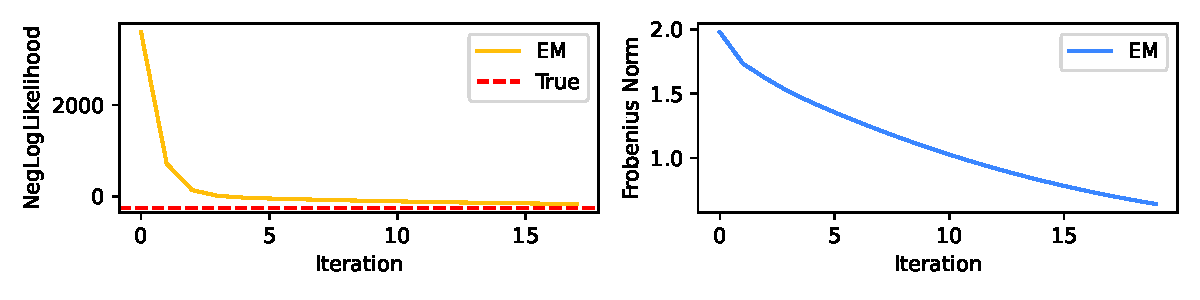
\includegraphics[width=\textwidth]{fig/H_neg_log_likelihood_fnorm.pdf}
    \caption{\(\mathbf{H}\) 的负对数似然与 Frobenius 范数变化。}
    \end{subfigure}
    \caption{EM 算法在估计 \(\mathbf{A}\)、\(\mathbf{Q}\) 和 \(\mathbf{H}\) 时的性能可视化结果。}
    \label{fig: exp car EM visualization}
\end{figure}

\begin{figure}[tb]
    \centering
    \begin{subfigure}[b]{0.85\textwidth}
        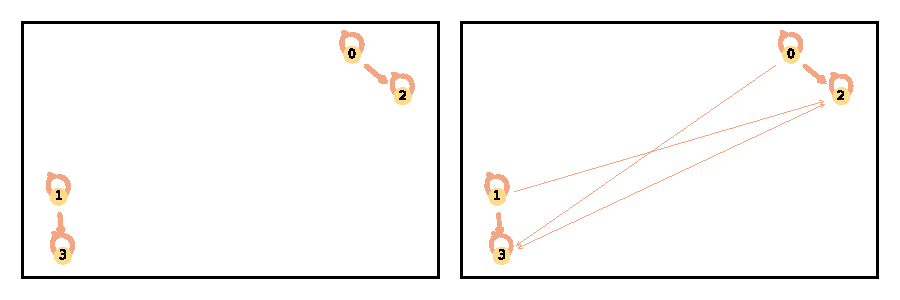
\includegraphics[width=\textwidth]{fig/A_graphs_for_true_and_EM.pdf}
        \caption{\(\mathbf{A}\) 的图结构表示:左为真实值,右为估计值。}
        \label{fig:subfig1}
    \end{subfigure}
    
    \begin{subfigure}[b]{0.85\textwidth}
        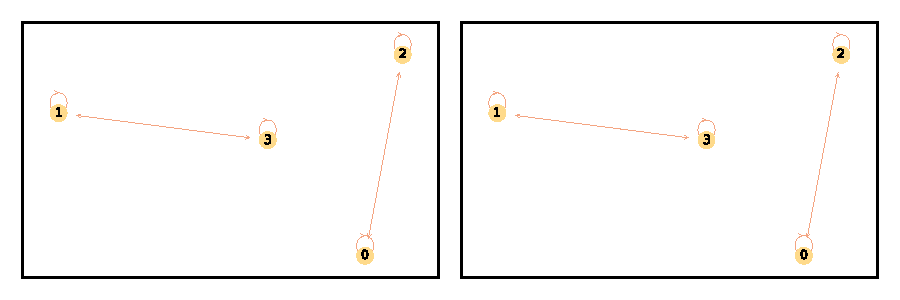
\includegraphics[width=\textwidth]{fig/Q_graphs_for_true_and_EM.pdf}
        \caption{\(\mathbf{Q}\) 的图结构表示:左为真实值,右为估计值。}
        \label{fig:subfig2}
    \end{subfigure}

    \begin{subfigure}[b]{0.85\textwidth}
    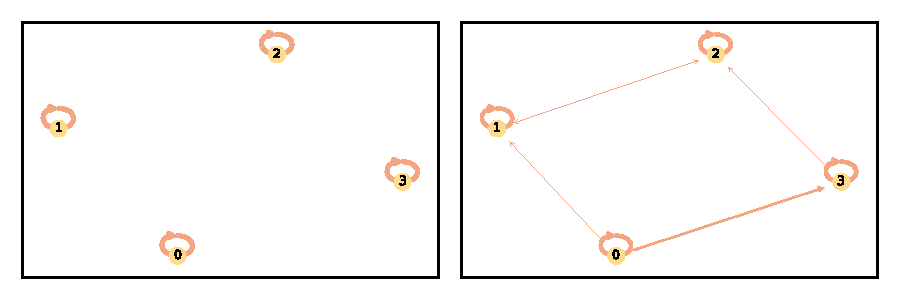
\includegraphics[width=\textwidth]{fig/H_graphs_for_true_and_EM.pdf}
    \caption{\(\mathbf{H}\) 的图结构表示:左为真实值,右为估计值。}
    \end{subfigure}
    \caption{真实参数与估计参数 \(\mathbf{A}\)、\(\mathbf{Q}\)、\(\mathbf{H}\) 的图形对比。}
    \label{fig: exp car graph comparison}
\end{figure}

为进一步直观展示参数估计过程,图~\ref{fig: exp car EM visualization} 展示了 EM 迭代中每个参数对应的负对数似然与 Frobenius 范数的变化趋势。此外,图~\ref{fig: exp car graph comparison} 给出了各参数的图结构对比图,分别显示了真实值与估计结果之间的差异。
    
\section{不同图结构下的正则化分析}

在本节中,我们介绍实验中使用的不同图结构的数学特性。这些结构在 GraphEM 算法中起到了定义转移矩阵正则化先验的关键作用。下文将对每种图类型进行详细分析,并说明其生成所采用的具体参数。

\paragraph*{分块对角结构(Blockwise-Diagonal)}
分块对角矩阵是一类特殊的稀疏矩阵,其非零元素局限于对角线上的若干块中。数学形式如下:
\[
\mathbf{A} = \begin{pmatrix}
\mathbf{A}_1 & \mathbf{0} & \cdots & \mathbf{0} \\
\mathbf{0} & \mathbf{A}_2 & \cdots & \mathbf{0} \\
\vdots & \vdots & \ddots & \vdots \\
\mathbf{0} & \mathbf{0} & \cdots & \mathbf{A}_k
\end{pmatrix},
\]
其中 \(\mathbf{A}_i\) 是子矩阵,\(\mathbf{0}\) 表示相应维度的零矩阵。该结构常用于建模解耦或弱耦合的子系统。

\paragraph*{小世界图(Small-World)}
小世界图具有较高的聚类系数与较短的平均路径长度。在实验中,我们使用 Watts-Strogatz 模型生成小世界图,设节点数 \(n = 16\),每个节点连接 \(k = 4\) 个最近邻节点,重连概率为 \(p = 0.3\)。小世界图的邻接矩阵 \(\mathbf{A}\) 通常具有局部连接与少量远程连接的混合特性,实现稀疏性与连通性的平衡。

\paragraph*{无标度图(Scale-Free)}
无标度图的节点度分布满足幂律形式:\(P(k) \sim k^{-\gamma}\),其中 \(k\) 是节点度,\(\gamma\) 是常数。我们使用 Barabási-Albert 模型生成无标度图,设 \(n = 16\),每步增加 \(m = 2\) 条边。该图的邻接矩阵 \(\mathbf{A}\) 高度稀疏,仅有少数枢纽节点具有较高的度数。

\paragraph*{二部图(Bipartite)}
二部图是一类可将顶点划分为两个不相交集合 \(U\) 与 \(V\) 的图,其中每条边仅连接 \(U\) 与 \(V\) 中的节点。实验中,我们生成一个完全二部图,节点数 \(n = 16\),两个子集分别为 \(n_1 = \lfloor n/2 \rfloor\)、\(n_2 = \lfloor n/2 \rfloor\)。其邻接矩阵形式如下:
\[
\mathbf{A} = \begin{pmatrix}
\mathbf{0} & \mathbf{B} \\
\mathbf{B}^\top & \mathbf{0}
\end{pmatrix},
\]
其中 \(\mathbf{B}\) 是表示两个集合间连接关系的矩阵。该结构适用于建模两个不同实体间的关联关系。

\paragraph*{环图(Cycle)}
环图由一个封闭的循环组成,每个节点恰好与两个其他节点相连。我们生成节点数为 \(n = 16\) 的环图。其邻接矩阵为循环矩阵(circulant matrix):
\[
\mathbf{A} = \begin{pmatrix}
0 & 1 & 0 & \cdots & 1 \\
1 & 0 & 1 & \cdots & 0 \\
0 & 1 & 0 & \cdots & 0 \\
\vdots & \vdots & \vdots & \ddots & \vdots \\
1 & 0 & 0 & \cdots & 0
\end{pmatrix}.
\]
环图常用于建模周期性或循环性结构。

\paragraph*{星型图(Star)}
星型图由一个中心节点与所有其他节点连接而成,其他节点之间没有连接。实验中,我们生成 \(n = 16\) 节点的星型图。其邻接矩阵为:
\[
\mathbf{A} = \begin{pmatrix}
0 & 1 & 1 & \cdots & 1 \\
1 & 0 & 0 & \cdots & 0 \\
1 & 0 & 0 & \cdots & 0 \\
\vdots & \vdots & \vdots & \ddots & \vdots \\
1 & 0 & 0 & \cdots & 0
\end{pmatrix}.
\]
星型图适用于建模中心化系统或星状网络结构(hub-and-spoke)。

\begin{table}[tb]
\centering
\caption{不同图结构在各类正则方法下的实验结果。每种图类型中加粗的数值表示最佳结果。}
\label{tab: prior results for block-diag}
\begin{tabular}{llll}
\toprule
\textbf{图类型} & \textbf{方法} & \textbf{\(\mathcal{L}_T(\widehat{\mathbf{A}})\)} & \textbf{\(\| \widehat{\mathbf{A}} - \mathbf{A} \|_F\)} \\
\midrule
分块对角 & EM & -21288.702 & 0.611 \\
 & GraphEM Laplace & -21262.253 & 0.575 \\
 & GraphEM Gaussian & -21287.225 & 0.608 \\
 & GraphEM Laplace+Gaussian & -21244.464 & \textbf{0.566} \\
小世界 & EM & -2237.305 & 2.489 \\
 & GraphEM Laplace & -2195.235 & 2.181 \\
 & GraphEM Gaussian & -2235.439 & 2.424 \\
 & GraphEM Laplace+Gaussian & -2193.343 & \textbf{2.140} \\
无标度 & EM & -2234.821 & 2.176 \\
 & GraphEM Laplace & -2197.950 & 2.005 \\
 & GraphEM Gaussian & -2233.167 & 2.138 \\
 & GraphEM Laplace+Gaussian & -2195.138 & \textbf{1.974} \\
二部图 & EM & -2228.962 & 2.366 \\
 & GraphEM Laplace & -2187.252 & 2.170 \\
 & GraphEM Gaussian & -2227.116 & 2.310 \\
 & GraphEM Laplace+Gaussian & -2185.598 & \textbf{2.127} \\
环图 & EM & -2279.460 & 2.257 \\
 & GraphEM Laplace & -2244.706 & 2.022 \\
 & GraphEM Gaussian & -2277.679 & 2.206 \\
 & GraphEM Laplace+Gaussian & -2243.051 & \textbf{1.984} \\
星型图 & EM & -2287.181 & 2.517 \\
 & GraphEM Laplace & -2253.640 & 2.240 \\
 & GraphEM Gaussian & -2285.723 & 2.456 \\
 & GraphEM Laplace+Gaussian & -2252.407 & \textbf{2.196} \\
\bottomrule
\end{tabular}
\end{table}

表~\ref{tab: prior results for block-diag} 总结了 EM 算法及其 GraphEM 变体(包括 Laplace、Gaussian 和 Laplace+Gaussian 正则化)在不同图结构上的性能表现,图类型包括分块对角、小世界、无标度、二部图、环图和星型图。表中报告了每种方法在每种图类型下的负对数似然 \(\mathcal{L}_T(\widehat{\mathbf{A}})\) 以及 Frobenius 范数 \(\| \widehat{\mathbf{A}} - \mathbf{A} \|_F\)。

从表中可以看出,GraphEM 的各类变体在 Frobenius 范数方面均优于标准 EM 算法。具体而言:
\begin{itemize}
    \item \textit{GraphEM Laplace+Gaussian} 方法在所有图类型中均表现最佳,取得了最小的 Frobenius 范数。这表明将 Laplace 与 Gaussian 先验结合能够提供更稳健的正则化框架。
    \item \textit{GraphEM Laplace} 方法相较标准 EM 同样具有显著提升,尤其在降低 Frobenius 范数方面效果明显,说明稀疏性正则化在刻画图结构方面是有效的。
    \item \textit{GraphEM Gaussian} 方法相比标准 EM 稍有提升,但整体效果不如 Laplace 及 Laplace \\ 
    + Gaussian 变体,进一步强调了诱导稀疏性的先验在图结构正则化中的重要性。
\end{itemize}

\begin{figure}[tb]
    \centering
    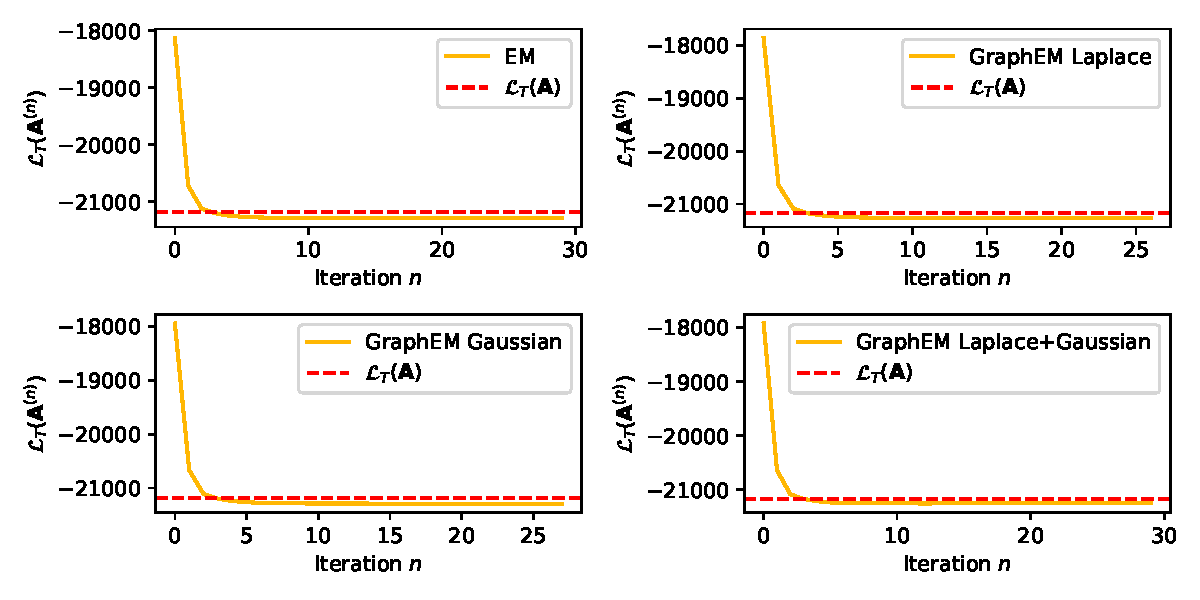
\includegraphics[width=0.85\linewidth]{fig/block diagonal/neg_log_likelihood.pdf}
    \caption{不同正则化方法下,分块对角图的负对数似然收敛曲线。}
    \label{fig: neg log likelihood}
\end{figure}

图~\ref{fig: neg log likelihood} 展示了分块对角图在不同正则方法下的负对数似然收敛情况。从图中可以看出,所有 EM 系列方法的收敛值均低于真实参数对应的负对数似然值,进一步验证了其估计效果的有效性。

\begin{figure}[tb]
    \centering
    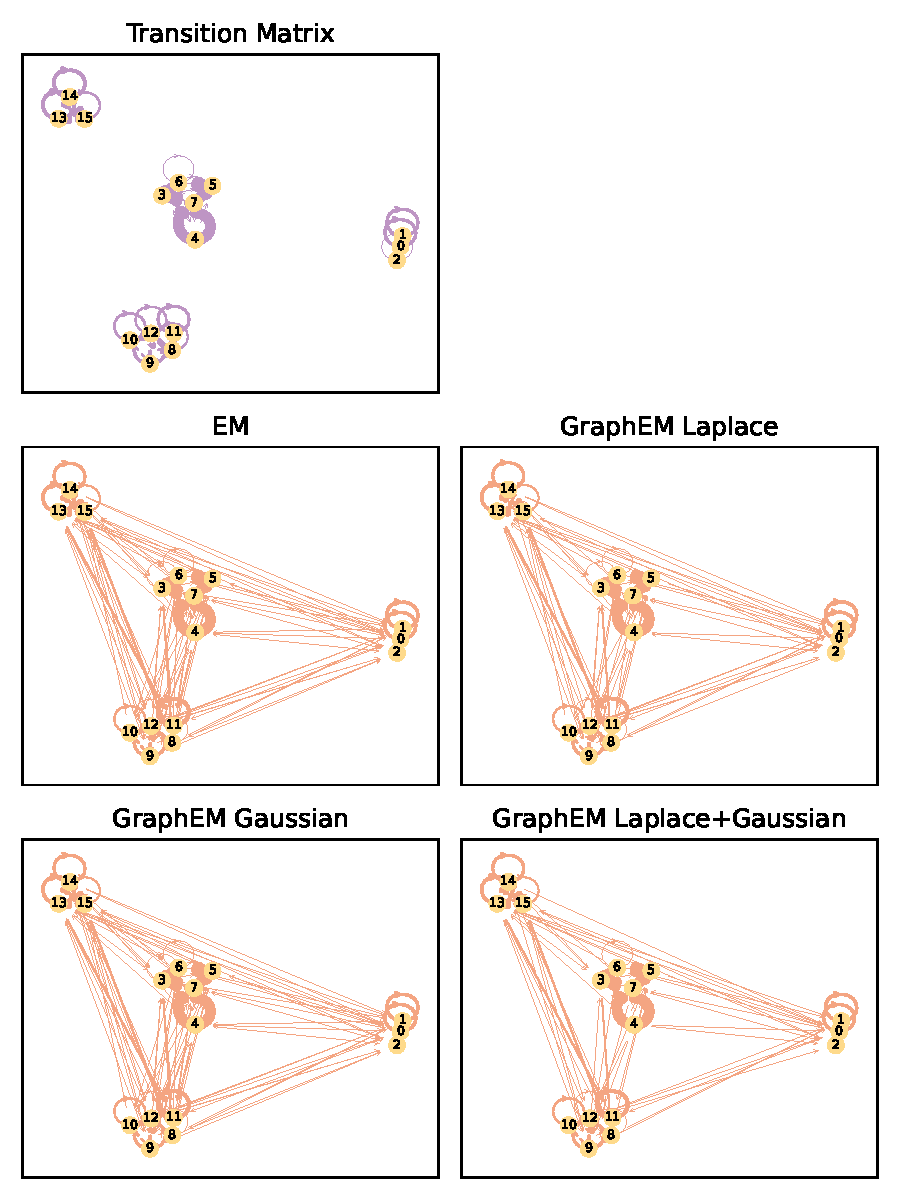
\includegraphics[width=0.75\linewidth]{fig/block diagonal/graphs_for_true_and_EM.pdf}
    \caption{分块对角图的真实转移矩阵与估计矩阵对比图。}
    \label{fig: graph comparison}
\end{figure}

为了进行更细致的对比,图~\ref{fig: graph comparison} 可视化展示了分块对角图的真实转移矩阵与估计转移矩阵。结果显示,GraphEM 的 Laplace 与 Laplace+Gaussian 方法所得估计最接近真实值,伪影更少,且更好地保留了块对角结构。

实验结果表明,将先验知识以正则化方式融入 EM 算法是有效的。具体而言:
\begin{itemize}
    \item \textit{Laplace 先验} 在促进稀疏性方面尤其有效,这对捕捉小世界图与无标度图等图结构至关重要。
    \item \textit{Gaussian 先验} 提供了更平滑的估计,但在保持稀疏性方面较弱,因此更适用于如二部图和环图这类相对稠密的结构。
    \item \textit{Laplace+Gaussian 先验} 综合了两种先验的优势,在所有图类型中表现最佳。这表明混合正则策略在图结构参数估计中具有高度通用性和效果。
\end{itemize}

这些发现突显了 GraphEM 在多种图结构上的优越性能。与标准 EM 算法相比,GraphEM 不仅保持了相当的收敛速度,而且在估计精度上有显著提升,进一步验证了其有效性。值得注意的是,在所有图类型中,在 Laplace 先验基础上引入 Gaussian 正则项的做法始终能进一步提升表现。这一现象可有两种解释:(1)稀疏性仍是这些图结构中的主导特征;或(2)算法对具体图类型具有一定鲁棒性。在这两种情形下,Gaussian 正则所引入的稳定性都能带来性能提升。

此外,我们还观察到,在 GraphEM 中将 Laplace 与 Gaussian 先验结合后,能够“无折中”地叠加两者的优点,而不会引入额外的优化计算开销。这一结果尤其具有前景意义,表明 GraphEM 的迭代优化框架可以无缝整合多种正则项。这一发现为未来研究开辟了新方向,即通过累积不同类型的正则项,在不增加计算复杂度的前提下迭代逼近最优解。

\newclearpage
% 论文后置部分
\backmatter
\renewcommand{\chaptermark}[1]{\markboth{\songti #1}{}}
% \chapter{结论}
% \label{cha:experiment}
% \section*{论文工作总结}
% ……
% \section*{工作展望}
% ……

\chapter{结论}

本文研究了 GraphEM 算法在线性高斯状态空间模型(LGSSM)参数估计中的应用。GraphEM 是一种新颖的算法,它将先验知识整合进期望最大化(EM)框架中。通过引入图推理与正则化技术,我们对原始 GraphEM 方法进行了扩展,使其能够处理更广泛的图结构与正则化策略,包括 Laplace、Gaussian 及混合 Laplace+Gaussian 先验。

一个具有前景的结果是,GraphEM 框架能够无缝集成多种正则项。Laplace 与 Gaussian 先验的组合实现了两者优势的“无折中”叠加,而不引入额外的优化开销。这一特性为未来的研究开辟了新方向:通过累积多样化的正则项,可以在不增加计算复杂度的前提下,迭代地逼近最优解。

% \section*{未来工作}

未来的研究方向包括发展自适应正则化策略,根据观测数据与图结构动态调整 Laplace 与 Gaussian 先验的权重。此外,进一步研究 GraphEM 在其他图类型上的表现,如随机图、分层图与动态图,有助于验证其通用性。对混合 Laplace+Gaussian 正则方法的收敛性与鲁棒性进行理论分析,也将有助于深入理解其有效性。最后,将 GraphEM 应用于金融、气候建模与社交网络分析等实际问题中,有望展示其在参数估计中的实用价值与潜在影响。
 % 制作结论章节
\newclearpage
% 参考文献
\makereferences % 制作参考文献
% 致谢
%%
% 致谢
% 谢辞应以简短的文字对课题研究与论文撰写过程中曾直接给予帮助的人员(例如指导教师、答疑教师及其他人员)表示对自己的谢意,这不仅是一种礼貌,也是对他人劳动的尊重,是治学者应当遵循的学术规范。内容限一页。
% modifier: 黄俊杰
% update date: 2017-04-15
%%

\chapter{致谢}

四年时光如白驹过隙,转眼间我的本科生活即将画上句点。回望这段时光,我不仅积累了丰富的知识与技能,更重要的是提升了我的分析和解决问题的能力,培养了良好的科学素养。虽然过程中走过一些弯路,但正是这些经历让我更加坚定了未来的方向,收获了许多宝贵的经验和教训。这一切的进步与成长,都离不开老师们的教诲和同学们的帮助,在此,我想向他们表达我最诚挚的谢意。

首先,我要特别感谢我的所有任课老师。在我还是一名本科生时,缺乏学术研究的经验,对于研究问题的重点、难点和热点往往难以把握,更难以评估自己的研究成果能够达到的层次。然而,老师们凭借他们渊博的知识和深刻的学术洞察力,给予了我无微不至的指导。这不仅在学术上给予了我明确的方向,帮助我理清思路,还在科研的过程中为我指引了正确的道路。他们严谨的治学态度、精益求精的工作作风,以及对学生的无私关怀,始终是我学习的榜样。在此,我想向老师们表达我最崇高的敬意和衷心的感谢,感谢他们在这段求学旅程中给予我的悉心指导和无私帮助。

其次,我要感谢我的同学们,特别是在研究过程中与我一同讨论、分享的伙伴们。大家在不同的学科领域中各具专长,在遇到问题时总能互相启发、共同解决。每一次的讨论和合作,不仅让我获得了新的知识,也让我深刻体会到团队合作的力量。你们的支持和鼓励是我不断进步的重要动力,在这里我要向你们表示最诚挚的感谢。

最后,我要深深感谢我的家人,是你们一直以来的无私奉献与默默支持,让我在面对困难和挑战时能够坚定信心、勇敢前行。你们给予我无限的爱与力量,使我能够在追求学术和个人成长的道路上不断超越自我,最终取得今天的成果。在此,我想对你们表达我最深沉的感激和爱。

四年的时光,虽然短暂,但每一步都充满了挑战与成长。感谢所有曾给予我帮助与支持的人,正是有了你们的陪伴,我才能走得更远、飞得更高。在未来的道路上,我将继续努力,不忘初心,勇敢追梦,回报这段珍贵的岁月。


\vskip 108pt
\begin{flushright}
    邓肯\makebox[1cm]{} \\
    \today
\end{flushright}

 % 制作致谢
\newclearpage
% 附录部分
% 附录
{
    \appendix
    \renewcommand{\chaptermark}[1]{\markboth{\songti  附录\thechapter\ ~#1}{}}
    % \chapter{补充更多细节}

% \section{补充图}

% \subsection{补充图}

% 这是附录内容,应该用宋体小四号字体。
% \begin{figure}[htbp]
%         \centering
%         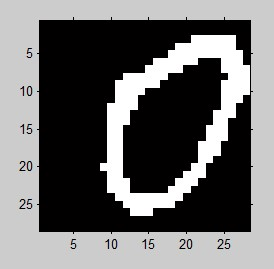
\includegraphics[height=6.54cm]{image/chap04/1.jpg}
%         \caption{实验训练集}
% \end{figure}
% \begin{figure}
%         \centering
%         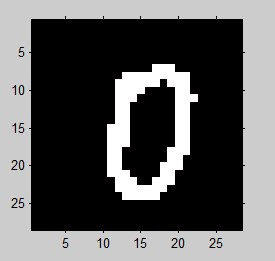
\includegraphics[height=6.54cm]{image/chap04/2.jpg}
%         \caption{实验测试集}
% \end{figure}

\chapter{其他图类型}

\paragraph*{小世界图(Small World)}
\begin{figure}[tb]
    \centering
    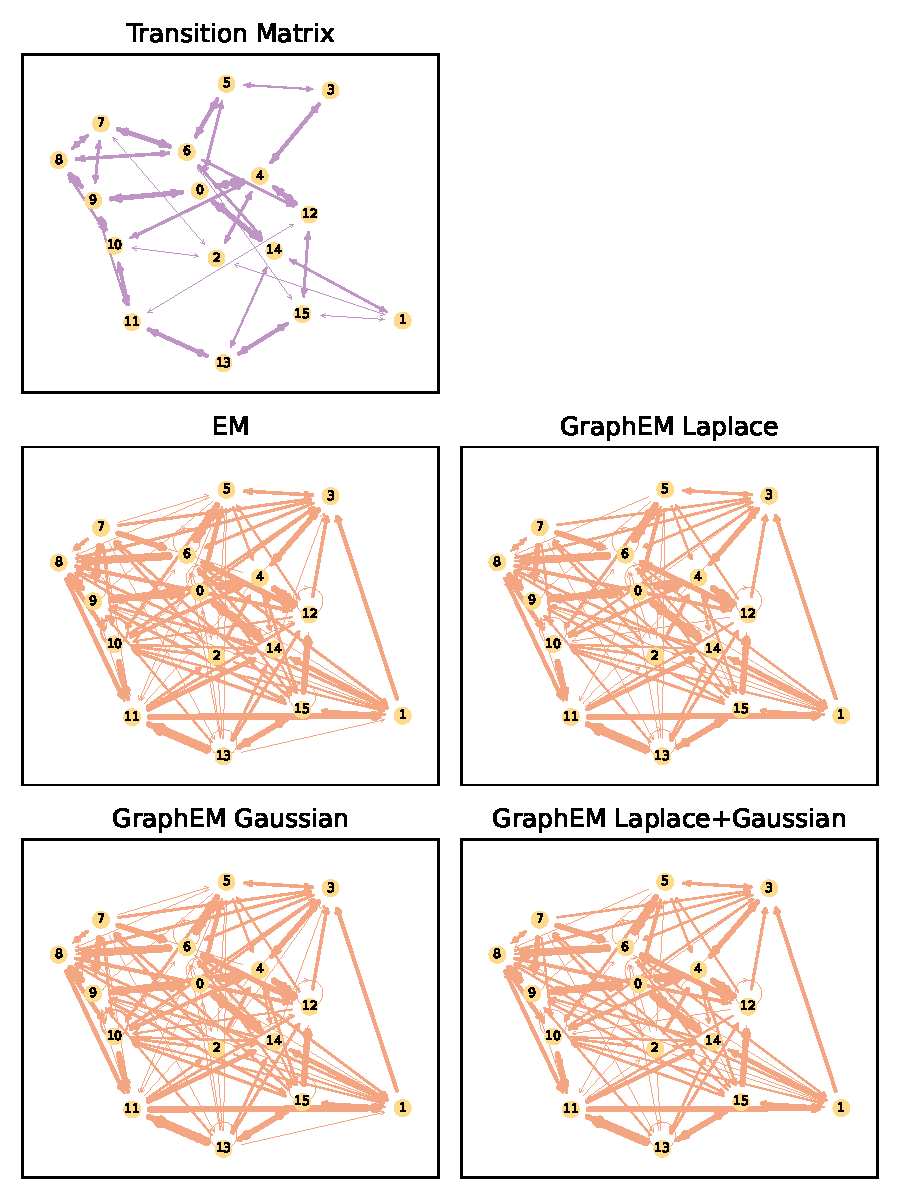
\includegraphics[width=0.75\linewidth]{fig/small world/graphs_for_true_and_EM.pdf}
    \caption{小世界图的真实转移矩阵与估计矩阵对比图。}
    \label{fig: small world graph comparison}
\end{figure}

图~\ref{fig: small world graph comparison} 对比了小世界图的真实转移矩阵与估计矩阵。结果表明,GraphEM 的 Laplace+Gaussian 方法能够有效捕捉小世界网络所特有的局部聚类与远程连接特性,其表现优于其他正则化策略。

\paragraph*{无标度图(Scale Free)}
\begin{figure}[tb]
    \centering
    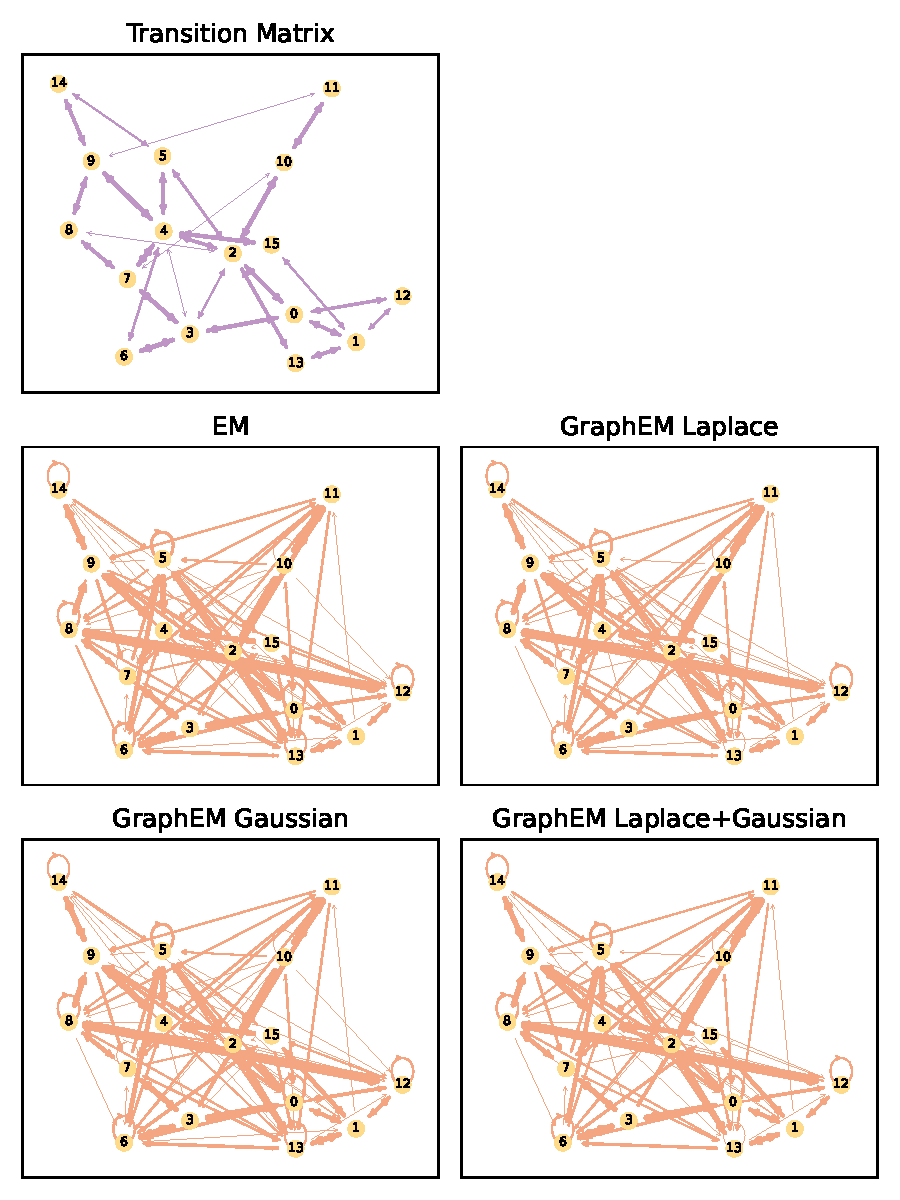
\includegraphics[width=0.75\linewidth]{fig/scale free/graphs_for_true_and_EM.pdf}
    \caption{无标度图的真实转移矩阵与估计矩阵对比图。}
    \label{fig: scale free graph comparison}
\end{figure}

图~\ref{fig: scale free graph comparison} 展示了无标度图的真实与估计转移矩阵。GraphEM Laplace+Gaussian 方法在识别枢纽节点和保持幂律度分布方面表现出色,显示出其在处理无标度结构时的鲁棒性。

\paragraph*{二部图(Bipartite)}
\begin{figure}[tb]
    \centering
    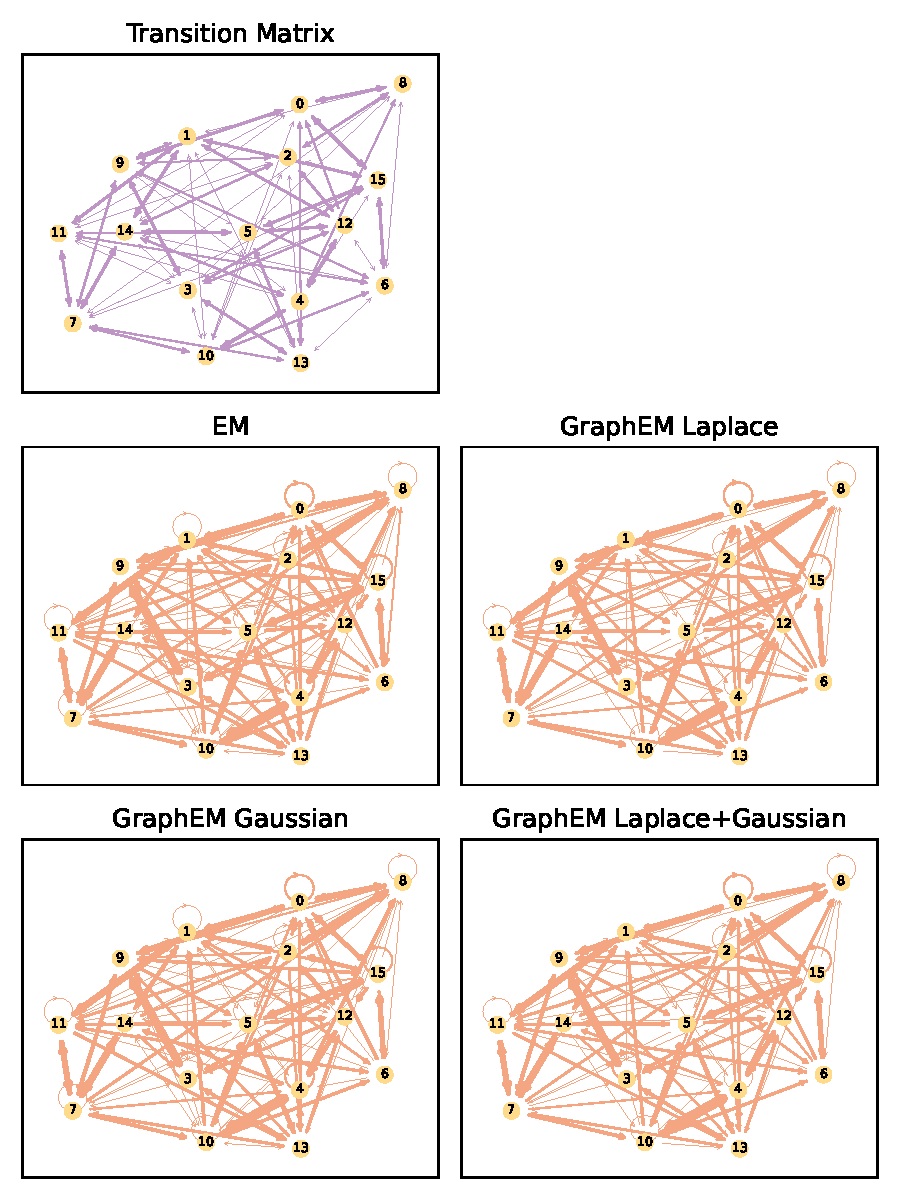
\includegraphics[width=0.75\linewidth]{fig/bipartite/graphs_for_true_and_EM.pdf}
    \caption{二部图的真实转移矩阵与估计矩阵对比图。}
    \label{fig: bipartite graph comparison}
\end{figure}

图~\ref{fig: bipartite graph comparison} 展示了二部图的真实与估计转移矩阵。GraphEM Laplace+Gaussian 方法能够准确捕捉二部结构,展现了其建模不同节点集合之间关系的能力。

\paragraph*{环图(Cycle)}
\begin{figure}[tb]
    \centering
    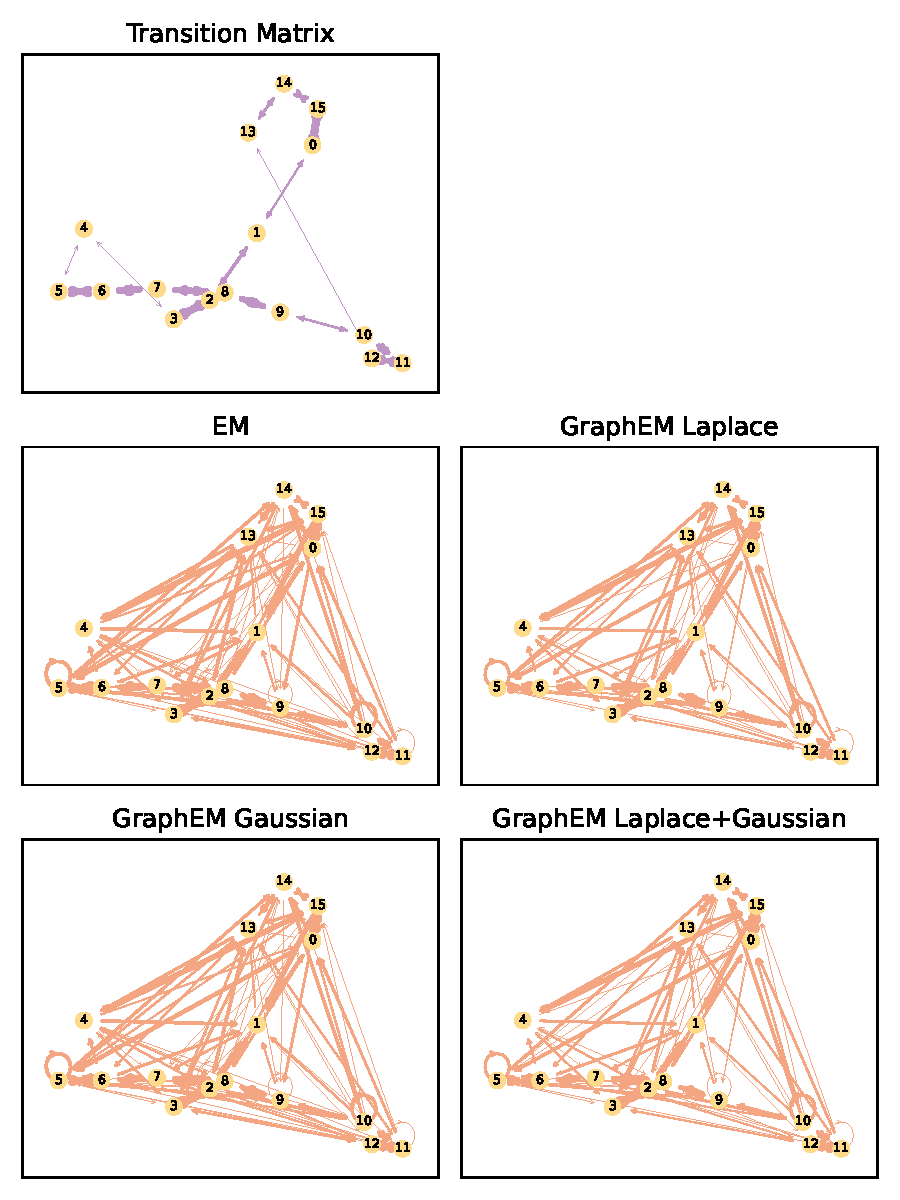
\includegraphics[width=0.75\linewidth]{fig/cycle/graphs_for_true_and_EM.pdf}
    \caption{环图的真实转移矩阵与估计矩阵对比图。}
    \label{fig: cycle graph comparison}
\end{figure}

图~\ref{fig: cycle graph comparison} 对比了环图的真实与估计转移矩阵。GraphEM Laplace+Gaussian 方法有效保留了环状结构,展现了其建模周期性关系的能力。

\paragraph*{星型图(Star)}
\begin{figure}[tb]
    \centering
    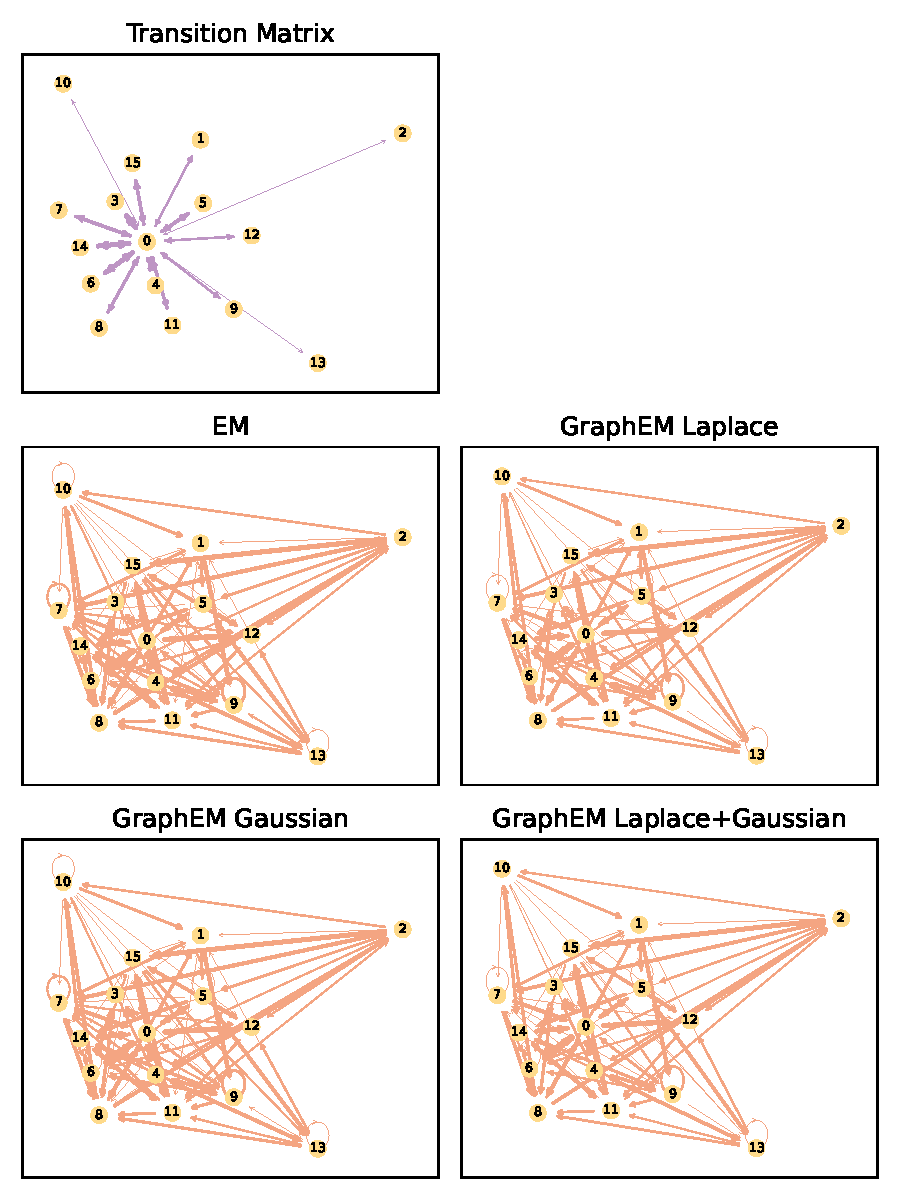
\includegraphics[width=0.75\linewidth]{fig/star/graphs_for_true_and_EM.pdf}
    \caption{星型图的真实转移矩阵与估计矩阵对比图。}
    \label{fig: star graph comparison}
\end{figure}

图~\ref{fig: star graph comparison} 展示了星型图的真实与估计转移矩阵。GraphEM Laplace+Gaussian 方法能够准确识别中心节点及其与边缘节点的连接,展现出其在建模星状网络中的有效性。

\endinput
 % 导入附录
    \newclearpage
}
\end{document}